\chapter{Implementation}\label{ch:impl}

This chapter describes the implementation of the Veritas toolchain. It presents the implementation of the core components---the source and target DTAL language, a type-preserving compiler, and an independent DTAL verifier---and the extensions made to them. It also presents the major extensions implemented: a borrowing and ownership model, region-backed array allocation, a compact runtime, and a bare-metal unikernel target. The chapter concludes by tracing a binary search program through the full pipeline as a worked example. 

\section{Repository overview}\label{sec:repo-overview}
%
The source code is organised as a single Rust crate with the following top-level module structure:
%
\begin{table}[h]
  \centering
  \begin{tabular}{l r l}
    \hline
    \textbf{Directory}                         & \textbf{Lines}  & \textbf{Responsibility}                     \\
    \hline
    \texttt{src/common/}                       & 788             & Shared AST, typed AST, and type definitions \\
    \texttt{src/frontend/}                     & 8,807           & Lexer, parser, and bidirectional type checker \\
    \texttt{src/backend/tir/}                  & 860             & Typed intermediate representation (SSA)     \\
    \texttt{src/backend/lower/}                & 2,322           & TAST to TIR lowering                        \\
    \texttt{src/backend/dtal/}                 & 2,740           & DTAL syntax, constraints, and parser        \\
    \texttt{src/backend/codegen/}              & 1,317           & TIR to DTAL code generation                 \\
    \texttt{src/backend/optimise/}             & 4,173           & Copy propagation and dead code elimination  \\
    \texttt{src/backend/regalloc/}             & 1,316           & Liveness analysis and allocators            \\
    \texttt{src/backend/physalloc.rs}          & 1,729           & Physical allocation and spill insertion     \\
    \texttt{src/backend/direct\_encode.rs}     & 386             & Direct physical-DTAL to x86-64 encoding     \\
    \texttt{src/backend/x86\_64/}              & 2,925           & Legacy x86-64 lowering and instruction forms \\
    \texttt{src/backend/elf/}                  & 531             & ELF generation, including bare-metal output \\
    \texttt{src/backend/runtime.rs}            & 177             & Hand-written runtime intrinsics             \\
    \texttt{src/backend/emit/}                 & 553             & DTAL text emitter                           \\
    \texttt{src/verifier/}                     & 7,817           & Independent DTAL verifier                   \\
    \texttt{src/main.rs}, \texttt{src/pipeline.rs}, module glue & 1,402 & CLI and pipeline orchestration              \\
    \hline
    \textbf{Total (excl.\ test-only modules)}  & \textbf{37,843} &                                             \\
    \hline
  \end{tabular}
  \caption{Repository structure and approximate line counts.}
  \label{tab:repo}
\end{table}

% \subsection{Usage}\label{sec:usage}

% Veritas programs are written in \texttt{.veri} source files. The compiler and verifier is invoked from the command line. Figure~\ref{fig:cli-help} shows the help output displayed after running \texttt{veritas --help}.
%
% \begin{figure}[H]
% \footnotesize
% \begin{verbatim}
% Veritas Compiler
%
% Usage: veritas <source_file> [OPTIONS]
%
% Output:
%   -o <file>            Compile to native ELF executable
%   --native             Print x86-64 assembly to stdout
%   --target-bare-metal  Generate Multiboot ELF for bare-metal/QEMU:
%                        qemu-system-x86_64 -kernel <binary> -serial stdio
%
% Verification:
%   --verify             Verify DTAL before code generation
%   --verify-only        Verify DTAL and exit (no codegen)
%   --verify-dtal        Verify a standalone .dtal file
%
% Optimisation:
%   -O, --optimize       Enable all optimisations
%
% Debug:
%   -v, --verbose        Show compilation stages
%   -q, --quiet          Suppress non-error output
%   --bench              Output benchmark JSON
%   -h, --help           Show this help message
% \end{verbatim}
% \caption{Veritas CLI help menu.}
% \label{fig:cli-help}
% \end{figure}


\section{Pipeline overview}

Figure~\ref{fig:pipeline} summarises the compilation pipeline. Each named representation is shown in sequence, and arrows indicate the transformations between them. Checked type annotations are preserved through TAST, TIR, and DTAL, and are no longer needed after DTAL verification and final encoding to x86-64.

\begin{figure}[h]
  \centering
  \begin{tcolorbox}[colback=white, colframe=black, width=\textwidth, boxrule=0.5pt]
    \begin{center}
      \texttt{Source} $\xrightarrow{\text{lex}}$ \texttt{Tokens} $\xrightarrow{\text{parse}}$ \texttt{AST} $\xrightarrow{\text{typecheck}}$ \texttt{\textcolor{blue}{TAST}} $\xrightarrow{\text{lower}}$ \texttt{\textcolor{blue}{TIR}} $\xrightarrow{\text{codegen}}$ \texttt{\textcolor{blue}{DTAL}} $\xrightarrow{\text{optimise}}$ \texttt{\textcolor{blue}{DTAL}} $\xrightarrow{\text{regalloc}}$ \texttt{\textcolor{blue}{DTAL}} $\xrightarrow{\text{encode}}$ \texttt{x86-64} $\xrightarrow{\text{encode}}$ \texttt{ELF}
    \end{center}
  \end{tcolorbox}
  \caption{The Veritas compilation pipeline. Representations carrying checked type annotations are in blue.}
  \label{fig:pipeline}
\end{figure}
%

\section{The Veritas language}\label{sec:source-language}

This section presents the syntax and formal typing rules of the Veritas source language. These define the contract that the compiler must uphold: any program accepted by the type checker satisfies the properties encoded in its types.

\subsection{Syntax}

The abstract syntax of Veritas is defined by the grammar in Figure~\ref{fig:veritas-syntax}.
% consider moving before rules
The metavariables used in the grammar are as follows: $n$ ranges over integer literals; $x$, $f$ range over identifiers (variables and function names); $N$ ranges over integer expressions that must reduce to a statically known constant (used for array sizes and singleton types). $P$ is the specification language used in refinement predicates, function contracts, and loop invariants, and additionally provides bounded quantifiers. A block $B$ is a sequence of zero or more statements followed by an optional trailing expression. If a block has a trailing expression, its value is the block's result; otherwise, its result is unit. Grey text denotes an optional clause; $(\cdot)^*$ denotes zero or more repetitions.

\begin{figure}[H]
{\small
\[
\renewcommand{\arraystretch}{1.09}
\begin{array}{@{}r@{\ }c@{\ }l@{\hspace{1.2em}}p{0.25\textwidth}@{}}
  T, \tau & ::= &
  \parbox[t]{0.66\textwidth}{
    $\textsf{unit} \,|\, \textsf{int} \,|\, \textsf{bool} \,|\, [T; N] \,|\, \textsf{int}(N) \,|\, \{ x:\textsf{int} \mid P \}$
  }
  & \textbf{(Types)} \\[2pt]
  c & ::= &
  \underline{n} \,|\, \textsf{true} \,|\, \textsf{false}
  & \textbf{(Base values)} \\[2pt]
  \textsf{aop} & ::= &
  \texttt{+} \,|\, \texttt{-} \,|\, \texttt{*} \,|\, \texttt{/} \,|\, \texttt{\%}
  \qquad \textsf{uaop} ::= \texttt{-}
  & \textbf{(Arithmetic operators)} \\[2pt]
  \textsf{cop} & ::= &
  \texttt{==} \,|\, \texttt{!=} \,|\, \texttt{<} \,|\, \texttt{<=} \,|\, \texttt{>} \,|\, \texttt{>=}
  & \textbf{(Comparison operators)} \\[2pt]
  \textsf{lop} & ::= &
  \texttt{\&\&} \,|\, \texttt{||} \,|\, \texttt{==>}
  \qquad \textsf{ulop} ::= \texttt{!}
  & \textbf{(Logical operators)} \\[2pt]
  e & ::= &
  \parbox[t]{0.66\textwidth}{
    $c \,|\, x \,|\, e \textsf{ aop } e \,|\, e \textsf{ cop } e \,|\, e \textsf{ lop } e \,|\, \textsf{ulop}\; e \,|\, \textsf{uaop}\; e \,|\, f(\overrightarrow{e}) \,|\, {}$\\
    $x[e_i] \,|\, \kw{if } e_\textsf{cond}\; \{B\}\; \kw{else } \{B'\} \,|\, [e_\textsf{val}; e_\textsf{size}]$
  }
  & \textbf{(Expressions)} \\[4pt]
  P & ::= &
  \parbox[t]{0.66\textwidth}{
    $e \textsf{ cop } e \,|\, P \textsf{ lop } P \,|\, \textsf{ulop}\; P \,|\, {}$\\
    $\kw{forall } x \kw{in } e_\textsf{start}..e_\textsf{end}\;\{P\} \,|\, \kw{exists } x \kw{in } e_\textsf{start}..e_\textsf{end}\;\{P\}$
  }
  & \textbf{(Propositions)} \\[4pt]
  S & ::= &
  \parbox[t]{0.66\textwidth}{
    $\kw{let } x:T = e; \,|\, \kw{let mut } x:T = e; \,|\, x = e; \,|\, x[e_i] = e; \,|\, \kw{return } e; \,|\, e; \,|\, {}$\\
    $\kw{if } e_\textsf{cond}\; \{B\}\; \kw{else } \{B'\} \,|\, \kw{if } e_\textsf{cond}\; \{B\} \,|\, {}$\\ 
    $\kw{for } x \kw{in } e_\textsf{start}..e_\textsf{end}\; \optclause{\textsf{invariant } P}\; \{B\} \,|\, \kw{while } e_\textsf{cond}\; \optclause{\textsf{invariant } P}\; \{B\}$
  }
  & \textbf{(Statements)} \\[4pt]
  D & ::= &
  \parbox[t]{0.66\textwidth}{
    $\kw{fn } f(x_1:T_1, \ldots)\; \rightarrow T_\textsf{ret}\; \optclause{\textsf{requires } P}\;\optclause{\textsf{ensures } P}\; \{B\}$
  }
  & \textbf{(Function definitions)} \\[2pt]
  \textsf{Prog} & ::= &
  D^*
  & \textbf{(Program)} \\[2pt]
  B & ::= &
  S^*\; \optclause{e}
  & \textbf{(Blocks)}
\end{array}
\]
}
\caption{Veritas' abstract syntax.}
\label{fig:veritas-syntax}
\end{figure}


\subsection{Typing contexts}\label{sec:typing-contexts}

The typing context is a tuple $(\phi, \Gamma, \Delta, \Sigma_F)$:

\begin{itemize}
    \item $\phi$: A set of refinement propositions known to be true (assumptions from branch conditions, preconditions, and refinement types).
    \item $\Gamma$: An immutable variable environment mapping names to types ($x : \tau$).
    \item $\Delta$: An environment for mutable variables mapping names to pairs of a \textit{current type} and a \textit{master type} ($x : (\tau_c, \tau_m)$). We write $(x: \tau_c) \in \Delta$ to extract the current type and $(x: \tau_m) \in \Delta$ for the master type.
    \item $\Sigma_F$: A global function signature environment.
\end{itemize}

\subsubsection{Master types}

The master type $\tau_m$ is set at declaration and never changes; the current type $\tau_c$ may be refined through control flow but must remain a subtype of $\tau_m$. To demonstrate: when a mutable variable is declared as \texttt{let mut x:T = e}, the type $T$ is recorded as the variable's master type $\tau_m$. The variable's \textit{current type} $\tau_c$ may be narrowed through assignments and control flow (e.g., after \texttt{if x > 0}, the current type narrows to $\{v\!:\!\mathtt{int} \mid v > 0\}$), but every assignment \texttt{x = e} must satisfy $\tau_e <: \tau_m$, where $\tau_e$ is the type synthesised for the right-hand-side expression $e$. At control-flow joins, current types from each branch are merged using the join operation, but the result must remain a subtype of the master type. This prevents the invalidation of refinements if \texttt{x} is reassigned. The interaction between master types and mutable variables is described in Section~\ref{sec:typechecker}.

\subsection{Context joining}\label{sec:context-joining}

At control-flow merge points (i.e., after \textbf{if-else} and loops), the typing contexts from each branch must be joined. The $\textsf{join}$ operation computes a least upper bound for each mutable variable's type and intersects the proposition sets:

\begin{itemize}
    \item Same singletons: $\textsf{int}(N) \sqcup \textsf{int}(N) = \textsf{int}(N)$.
    \item Different singletons: $\textsf{int}(N_1) \sqcup \textsf{int}(N_2) = \textsf{int}$ where $N_1 \ne N_2$ (widen to base type).
    \item Refined types: $\{v \mid P\} \sqcup \{v \mid Q\} = \{v \mid P \vee Q\}$ (disjoin predicates).
    \item Singleton and refined: promote the singleton to $\{v \mid v = N\}$, then disjoin with the refined type's predicate.
    \item Refined and unrefined: $\{v \mid P\} \sqcup \textsf{int} = \textsf{int}$ (widen to base type).
    \item Arrays: read-only element facts may join as $[\tau_1; N] \sqcup [\tau_2; N] = [\tau_1 \sqcup \tau_2; N]$; mutable array bindings retain their declared writable type and stores update versioned array facts.
    \item Propositions ($\phi$): intersect (keep only propositions provable in both branches).
\end{itemize}

\noindent When $\textsf{join}$ is used in expression rules (e.g., \textsc{T-If-Expr}), the same type-joining rules apply to the result types of both branches.

\subsection{Judgement forms}\label{sec:judgement-forms}

Throughout the typing rules, $\tau$ is used as the metavariable for types.

The type system uses the following bidirectional typing judgements:

\begin{itemize}
    \item \textbf{Synthesis:} $\phi; \Delta; \Gamma \vdash e \Rightarrow (\phi'; \Delta'; \tau)$ --- synthesise type $\tau$ for expression $e$, potentially updating the context.
    \item \textbf{Checking:} $\phi; \Delta; \Gamma \vdash e \Leftarrow \tau : (\phi'; \Delta')$ --- check that $e$ has type $\tau$.
    \item \textbf{Subtyping:} $\phi \vdash \tau_1 <: \tau_2$ --- $\tau_1$ is a subtype of $\tau_2$ under assumptions $\phi$.
    \item \textbf{Provability:} $\phi \vdash P$ --- proposition $P$ is valid under assumptions $\phi$ (decided by SMT).
\end{itemize}

The checking and synthesis judgements are connected by a subsumption rule:
% If an expression synthesises type $\tau_e$ and the expected type is $\tau$, checking succeeds when $\tau_e <: \tau$:

$$\frac{\phi; \Delta; \Gamma \vdash e \Rightarrow (\phi'; \Delta'; \tau_e) \quad \phi' \vdash \tau_e <: \tau}{\phi; \Delta; \Gamma \vdash e \Leftarrow \tau : (\phi'; \Delta')} \quad (\textsc{T-Sub})$$

\subsection{Subtyping rules}

The subtyping relation $\phi \vdash \tau_1 <: \tau_2$ is defined by structural rules (listed in full in Appendix~\ref{app:source-rules}) and two rules that invoke the SMT solver. Mutable arrays are treated invariantly in the checked fragment; covariant element reasoning is used only for read-only facts. In both solver-backed rules, the propositions in $\phi$ are asserted as assumptions, the goal is negated, and the solver is checked for unsatisfiability:

$$\frac{\phi \vdash P[N/x]}{\phi \vdash \textsf{int}(N) <: \{x: \textsf{int} \mid P\}} \quad (\textsc{Sub-Singleton-Refine})$$

$$\frac{\phi \wedge P_1 \vdash P_2}{\phi \vdash \{x: \textsf{int} \mid P_1\} <: \{x: \textsf{int} \mid P_2\}} \quad (\textsc{Sub-Refine-Refine})$$

\subsection{Expression typing rules}\label{sec:expr-typing-rules}

For expressions whose value is used in a proof obligation, synthesis returns both a type and an SMT-level index term:
\[
  \phi;\Delta;\Gamma \vdash e \Rightarrow (\phi';\Delta';\tau;\iota)
\]
The term $\iota$ denotes the expression's value in generated constraints. For a singleton it is the singleton index; for a refinement or existential type it is the symbolic term introduced during synthesis, not merely the binder name in the refinement. Boolean expressions also expose a guard proposition $\mathsf{guard}(e)$, for example $\mathsf{guard}(e_1 < e_2) = \iota_1 < \iota_2$. Conditional and loop rules use this guard, so branch facts such as \texttt{lo <= hi} enter the corresponding path context.

Arithmetic operations use a $\textsf{join-op}$ function that performs constant folding when both operands are singletons (e.g., $\textsf{join-op}(+, \textsf{int}(1), \textsf{int}(2)) = \textsf{int}(3)$) and otherwise synthesises a refinement type via SMT refinement synthesis (e.g., $\{v\!:\!\textsf{int} \mid v = e_L + e_R\}$):

$$
  \frac{
    \begin{array}{c}
      \phi_0; \Delta_0; \Gamma \vdash e_L \Rightarrow (\phi_1; \Delta_1; \tau_L; \iota_L) \quad \phi_1 \vdash \tau_L <: \textsf{int} \\
      \phi_1; \Delta_1; \Gamma \vdash e_R \Rightarrow (\phi_2; \Delta_2; \tau_R; \iota_R) \quad \phi_2 \vdash \tau_R <: \textsf{int} \\
      \textsf{arith-safe}(\textsf{aop}, \iota_L, \iota_R, \phi_2) \quad
      \tau_\textsf{res} = \textsf{join-op}(\textsf{aop}, \tau_L, \tau_R)
    \end{array}
  }{
    \phi_0; \Delta_0; \Gamma \vdash e_L \textsf{ aop } e_R \Rightarrow (\phi_2; \Delta_2; \tau_\textsf{res}; \iota_L \textsf{ aop } \iota_R)
  } \quad (\textsc{T-Op})
$$

\noindent $\textsf{arith-safe}$ requires non-zero divisors for division and modulo and includes the signed-64-bit range obligations that the current implementation checks. Arithmetic outside those emitted side conditions is not part of the scoped guarantee.

Array indexing requires a bounds proof obligation, verified by the SMT solver:

$$
  \frac{
    \begin{array}{c}
      (x: [\tau_\textsf{elem}; N]) \in (\Gamma \cup \Delta_0)                                                                              \\
      \phi_0; \Delta_0; \Gamma \vdash e_i \Rightarrow (\phi_1; \Delta_1; \tau_i; \iota_i) \quad \phi_1 \vdash \tau_i <: \textsf{int} \\
      \phi_1 \vdash 0 \le \iota_i < N \quad \text{(Bounds proof)}
    \end{array}
  }{
    \phi_0; \Delta_0; \Gamma \vdash x[e_i] \Rightarrow (\phi_1; \Delta_1; \tau_\textsf{elem}; \textsf{select}(x,\iota_i))
  } \quad (\textsc{T-Array-Idx})
$$

Conditional expressions check both branches under the condition and its negation, then join the resulting contexts:
% using the $\textsf{join}$ operation defined in Section~\ref{sec:context-joining}

$$
  \frac{
    \begin{array}{c}
      \phi_0; \Delta_0; \Gamma \vdash e_\textsf{cond} \Rightarrow (\phi_1; \Delta_1; \tau_c) \quad \phi_1 \vdash \tau_c <: \textsf{bool} \\
      P_c = \mathsf{guard}(e_\textsf{cond}) \\
      \phi_1 \wedge P_c; \Delta_1; \Gamma \vdash B \Rightarrow (\phi_2; \Delta_2; \tau_2)                      \\
      \phi_1 \wedge \neg P_c; \Delta_1; \Gamma \vdash B' \Rightarrow (\phi_3; \Delta_3; \tau_3)                \\
      (\phi_\textsf{join}, \Delta_\textsf{join}, \tau_\textsf{join}) = \textsf{join}(\phi_2, \Delta_2, \tau_2, \phi_3, \Delta_3, \tau_3)
    \end{array}
  }{
    \phi_0; \Delta_0; \Gamma \vdash (\textsf{if } e_\textsf{cond}\; B \textsf{ else } B') \Rightarrow (\phi_\textsf{join}; \Delta_\textsf{join}; \tau_\textsf{join})
  } \quad (\textsc{T-If-Expr})
$$

Function calls verify argument types and the precondition (a proof obligation discharged by the SMT solver):

$$
  \frac{
    \begin{array}{c}
      \Sigma_F(f) = ( (x_i:\tau_i)_{i=1}^k \rightarrow \tau_\textsf{ret}\; \textsf{requires } P_\textsf{req} )                                  \\
      \phi_0; \Delta_0; \Gamma \vdash \vec{e} \Rightarrow (\phi_k; \Delta_k; \vec{\sigma}; \vec{\iota}) \\
      \forall i \in 1..k,\; \phi_k \vdash \sigma_i <: \tau_i                                                \\
      \phi_k \vdash P_\textsf{req}[\vec{\iota} / \vec{x}] \quad \text{(Precondition proof)}
    \end{array}
  }{
    \phi_0; \Delta_0; \Gamma \vdash f(\vec{e}) \Rightarrow (\phi_k; \Delta_k; \tau_\textsf{ret})
  } \quad (\textsc{T-Call})
$$

\subsection{Statement typing rules}\label{sec:stmt-typing-rules}

Standard rules for blocks, let bindings, array assignment, if-statements, and while loops are given in Appendix~\ref{app:source-rules}. Some of the more interesting rules are described below.

Assignment checks that the new value conforms to the master type:

$$
  \frac{
    \begin{array}{c}
      (x: \tau_m) \in \Delta_0 \\
      \phi_0; \Delta_0; \Gamma \vdash e \Rightarrow (\phi_1; \Delta_1; \tau_e)  \\
      \phi_1 \vdash \tau_e <: \tau_m
    \end{array}
  }{
    \phi_0; \Delta_0; \Gamma \vdash (x = e;) : (\phi_1; \Delta_1[x \mapsto (\tau_e, \tau_m)]; \Gamma)
  } \quad (\textsc{T-Assign})
$$

For loops bind the loop variable to the immutable context with bound propositions added to $\phi$, and require the loop invariant (if present) to hold on entry and be preserved by the body. The invariant is checked at entry by substituting $e_\textsf{start}$ for $i$, and preservation is checked after the body by substituting $i + 1$ for $i$:

$$
  \frac{
  \begin{array}{c}
    \phi_0 \wedge P_I[e_\textsf{start}/i] \quad \text{(Invariant holds on entry)} \\
    \phi_0 \wedge P_I \wedge e_\textsf{start} \le i < e_\textsf{end};\; \Delta_0;\; (\Gamma, i: \textsf{int}) \vdash B : (\phi_1; \Delta_1; \Gamma) \\
    \phi_1 \vdash P_I[(i+1)/i] \quad \text{(Invariant preserved by body)}
  \end{array}
  }{
  \phi_0; \Delta_0; \Gamma \vdash (\textsf{for } i \textsf{ in } e_\textsf{start}..e_\textsf{end}\;\{B\}) : (\phi_0 \wedge P_I; \Delta_0; \Gamma)
  } \quad (\textsc{T-For})
$$

\noindent where $P_I$ is the invariant proposition (or $\top$ if no invariant is specified).

\subsection{Function contracts}

Programmers may declare preconditions ($\mathbf{requires}\ P$) and postconditions ($\mathbf{ensures}\ P$) on functions, where $P$ is a proposition that may reference parameters and (for postconditions) the special variable $\mathtt{result}$.

At each call site, the type checker verifies $\phi \vdash P_\textsf{req}[\overline{e_i/x_i}]$: the precondition with actual argument expressions substituted for formal parameters (see rule \textsc{T-Call}). At each \textsf{return} statement, the return expression is synthesised, checked against the declared return type, and the postcondition is verified:

$$
  \frac{
    \begin{array}{c}
      \phi_0; \Delta_0; \Gamma \vdash e \Rightarrow (\phi_1; \Delta_1; \tau_e) \quad \phi_1 \vdash \tau_e <: \tau_\textsf{ret} \\
      \phi_1 \vdash P_\textsf{ens}[e/\mathtt{result}] \quad \text{(Postcondition proof)}
    \end{array}
  }{
    \phi_0; \Delta_0; \Gamma \vdash (\textsf{return } e;) : (\phi_1; \Delta_1; \Gamma)
  } \quad (\textsc{T-Return})
$$

\subsection{Quantified specifications}

The constraint language supports bounded quantifiers and implication to express properties over finite program ranges. Quantifiers may only appear in specification positions (preconditions, postconditions, refinement predicates), not in runtime code; the type checker enforces this restriction.

An important feature is \textit{refinement lifting}: an array typed as $[\{v\!:\!\textsf{int} \mid v \ge 0\}; N]$ automatically satisfies the quantified constraint $\forall i \in [0, N).\; \mathit{arr}[i] \ge 0$. This is achieved by extracting a quantified proposition from the array's element type and adding it to the context when the array is in scope.

\section{The DTAL target language}\label{sec:dtal-target-lang}

Veritas targets a first-order variant of Xi and Harper's DTAL design~\cite{Xi2001DTAL}. In their original work, Xi and Harper formally established the soundness of DTAL, proving that well-typed programs cannot violate memory safety or the constraints of the type system.
% the compiler emits DTAL annotated with type information, and a standalone verifier re-derives the types from scratch. If the compiler introduces an error, the annotations will be inconsistent and the verifier will reject the program. 
This section describes the concrete instruction set and typing judgements of V-DTAL, which builds on the theoretical foundation of DTAL.

\subsection{Instruction set}\label{sec:dtal-instr-set}

The DTAL instruction set resembles a standard RISC assembly language but is augmented with type annotations and constraint assertions. DTAL appears in two forms in the pipeline: a virtual-register form emitted by code generation, and a physical-register form produced after register allocation. Both carry verifier-facing type information, and the final verifier checks the physical form. The core syntax is summarised in Figure~\ref{fig:dtal-syntax}.

\begin{figure}[H]
{\small
\[
\renewcommand{\arraystretch}{1.09}
\begin{array}{@{}r@{\ }c@{\ }l@{\hspace{1.2em}}p{0.25\textwidth}@{}}
  R & ::= &
  r \mid v
  & \textbf{(Registers)} \\[2pt]
  e_i & ::= &
  \parbox[t]{0.66\textwidth}{
    $n \,|\, R \,|\, e_i + e_i \,|\, e_i - e_i \,|\, e_i \times e_i \,|\, e_i \div e_i \,|\, e_i \bmod e_i \,|\, \textsf{select}(R, e_i)$
  }
  & \textbf{(Index expressions)} \\[4pt]
  C & ::= &
  \parbox[t]{0.66\textwidth}{
    $e_i \textsf{ cop } e_i \,|\, C \textsf{ lop } C \,|\, \neg C \,|\, {}$\\
    $\textsf{forall } x \textsf{ in } e_i..e_i.\; C \,|\, \textsf{exists } x \textsf{ in } e_i..e_i.\; C$
  }
  & \textbf{(Constraints)} \\[4pt]
  \tau & ::= &
  \parbox[t]{0.66\textwidth}{
    $\textsf{unit} \,|\, \textsf{int} \,|\, \textsf{i64} \,|\, \textsf{bool} \,|\, [\tau; e_i] \,|\, {}$\\
    $\textsf{int}(e_i) \,|\, \{x:\textsf{int} \mid \varphi(x)\} \,|\, \exists x.\; \textsf{int}(x)\; \textsf{where}\; \varphi(x)$
  }
  & \textbf{(Types)} \\[4pt]
  d & ::= &
  \parbox[t]{0.66\textwidth}{
    $\texttt{.function } f \,|\, \texttt{.params } \Gamma \,|\, \texttt{.returns } \tau \,|\, \texttt{.precondition } C \,|\, {}$\\
    $\texttt{.postcondition } C \,|\, \texttt{.entry } \Gamma \,|\, \texttt{.assume } C \,|\, {}$\\
    $\texttt{.assert } C \,|\, \texttt{type } R : \tau$
  }
  & \textbf{(Directives)} \\[4pt]
  \iota & ::= &
  \parbox[t]{0.66\textwidth}{
    $\texttt{mov } R_d, R_s : \tau \,|\, \texttt{mov } R_d, n : \tau \,|\, \texttt{binop } R_d, R_1, R_2 : \tau \,|\, {}$\\
    $\texttt{addimm } R_d, R_s, n : \tau \,|\, \texttt{not } R_d, R_s : \tau \,|\, {}$\\
    $\texttt{load } R_d, [R_b + R_i] : \tau \,|\, \texttt{store } [R_b + R_i], R_s \,|\, {}$\\
    $\texttt{cmp } R_1, R_2 \,|\, \texttt{cmp } R_1, n \,|\, \texttt{setcc } R_d, cc : \tau \,|\, {}$\\
    $\texttt{jmp } L \,|\, \texttt{branch } cc, L \,|\, \texttt{call } f \,|\, \texttt{ret} \,|\, {}$\\
    $\texttt{push } R_s \,|\, \texttt{pop } R_d : \tau \,|\, \texttt{alloca } R_d, n : \tau$
  }
  & \textbf{(Instructions)} \\[4pt]
  B & ::= &
  L :\; d^*\; \iota^*
  & \textbf{(Blocks)} \\[2pt]
  F & ::= &
  d^*\; B^*
  & \textbf{(Functions)}
\end{array}
\]
}
\caption{Core V-DTAL syntax. Here $v$ ranges over virtual registers, $r$ over physical registers, $R$ over either kind of register, $L$ over labels, and $\Gamma$ over register type states.}
\label{fig:dtal-syntax}
\end{figure}

\noindent The annotation instructions are the distinguishing feature of DTAL. Destination-producing instructions carry type annotations where needed, and \texttt{type} and \texttt{assert} annotations embed additional verification evidence directly into the instruction stream. These annotations record facts such as bounds proofs and loop invariants.

% After register allocation, additional physical instructions are emitted (\texttt{prologue}, \texttt{epilogue}, spill loads/stores, \texttt{cqo}/\texttt{idiv} for division) which are verified but not relevant to the formal typing rules. Crucially, the independent verifier operates on this post-regalloc \textit{physical} DTAL rather than the virtual-register SSA form, meaning it also validates the correctness of register allocation and spilling. This strengthens the safety guarantee: the register allocator, like the rest of the compiler, is untrusted.

\subsection{DTAL directives}

In addition to executable instructions, the textual DTAL format contains directives that describe function metadata, block entry states, and verifier annotations. Figure~\ref{fig:dtal-directives} shows where these directives appear in a typical DTAL function.

\begin{figure}[H]
\centering
\footnotesize
\begin{verbatim}
.function f
.params {r0: int, r1: [int; 10]}       ; function inputs
.returns int                           ; return type
.precondition r0 >= 0                  ; optional caller obligation
.postcondition result >= 0             ; optional return guarantee

f:
.f_bb0:
    .entry {r0: int, r1: [int; 10]}    ; expected block-entry state
    .assume r0 >= 0                    ; block-entry constraint
    cmp r0, 10
    bge .f_exit

.f_body:
    .entry {r0: {v: int | v < 10}, r1: [int; 10]}
    load r2, [r1 + r0]    : int
    .assert r2 >= 0                    ; checked before use downstream
    ret

.f_exit:
    .entry {r0: int, r1: [int; 10]}
    ret
\end{verbatim}
\caption{DTAL directives describe function signatures, block entry states, and verifier constraints; ordinary instructions perform computation.}
\label{fig:dtal-directives}
\end{figure}

Function-level directives define the verifier-facing signature and contract. Block-level directives declare the type state that must hold when control enters a block, and edge checking proves that predecessor states imply these entry states. Constraint directives split into assumptions, which form part of the declared block state, and assertions, which are checked at their program point before being added to the context. Physical directives such as \texttt{.prologue} and \texttt{.epilogue} appear only after register allocation.

\subsection{DTAL type system}

The DTAL type system largely mirrors the source-level type system: it retains unit, integer and boolean base types, machine-integer types, singleton integers $\textsf{int}(N)$, refinement types, arrays, and master types. The main difference is that these types classify \emph{registers} rather than source variables, so the indices appearing in types are low-level expressions over register contents. In particular, DTAL index expressions may mention constants, register names, arithmetic, and $\textsf{select}(\mathit{arr}, i)$ for array element access (of an array $\mathit{arr}$ atindex $i$).

The most important addition is the use of \textit{existential types} to represent results that are known only symbolically at the assembly level. When arithmetic on non-singleton operands cannot preserve an exact singleton type, the result is represented as an existential such as $\exists x.\; \textsf{int}(x) \;\mathbf{where}\; \varphi(x)$, where $\varphi$ is a predicate over integer witnesses. This allows the verifier to retain enough logical structure for later proof obligations without requiring every intermediate value to have a concrete singleton type.

The DTAL constraint language preserves the same core logical fragment used in source-level specifications: comparisons, logical connectives, and bounded quantifiers. However, it is represented separately as a first-order language over DTAL index expressions rather than directly as source expressions, and conversion from source expressions to this constraint language is partial. These constraints are threaded through the verifier's type state and refined by comparisons, branches, assertions, and function contracts.

\subsection{DTAL typing judgements}

DTAL type checking operates over a \textit{type state}. The rules below show the core part of this state as $(\Phi, \Gamma)$, where $\Gamma$ maps registers to their current types and $\Phi$ is a set of constraints known to hold at a given program point. The implementation also records auxiliary verifier state such as the comparison/flag state $\mathcal{F}$, the typed stack, array versions, spill slots, and proven assertions. The core judgement for instruction typing is $\Phi; \Gamma \vdash \textsf{instr} \Rightarrow \Gamma'$, meaning that executing $\textsf{instr}$ under constraints $\Phi$ and register state $\Gamma$ produces a new register state $\Gamma'$. Rules that read or update machine-flag state use $\Phi; \Gamma; \mathcal{F} \vdash \textsf{instr} \Rightarrow \Gamma'; \mathcal{F}'$.

\paragraph{Move Immediate}
Loading a constant into a register assigns it a singleton type:
$$
\frac{}{\Phi; \Gamma \vdash \textsf{mov } r_d, n \Rightarrow \Gamma[r_d \mapsto \textsf{int}(n)]} \quad (\textsc{D-MovImm})
$$

\paragraph{Arithmetic}
When both operands have singleton types, the result is a singleton capturing the exact value. In the general case (refined or existential operands), the result is an existential type:
$$
\frac{\Gamma(r_1) = \textsf{int}(e_1) \quad \Gamma(r_2) = \textsf{int}(e_2)}{\Phi; \Gamma \vdash \textsf{add } r_d, r_1, r_2 \Rightarrow \Gamma[r_d \mapsto \textsf{int}(e_1 + e_2)]} \quad (\textsc{D-BinOp-Singleton})
$$

$$
\frac{
  \begin{array}{c}
    \Gamma(r_1) = \{a\!:\!\textsf{int} \mid \varphi_1(a)\} \quad \Gamma(r_2) = \{b\!:\!\textsf{int} \mid \varphi_2(b)\} \\
    \varphi_+(c) = \exists a,b.\; \varphi_1(a) \wedge \varphi_2(b) \wedge c = a + b
  \end{array}
}{\Phi; \Gamma \vdash \textsf{add } r_d, r_1, r_2 \Rightarrow \Gamma[r_d \mapsto \exists c.\; \textsf{int}(c) \;\mathbf{where}\; \varphi_+(c)]} \quad (\textsc{D-BinOp-Refined})
$$

\paragraph{Memory Access (Bounds Checking)}
A memory load is only well-typed if $\Phi$ can prove that the index is within bounds. The result type is the array's element type:
$$
\frac{\Gamma(r_b) = [\tau; N] \quad \Phi \vdash 0 \le e_i < N}{\Phi; \Gamma \vdash \textsf{load } r_d, [r_b, r_i] \Rightarrow \Gamma[r_d \mapsto \tau]} \quad (\textsc{D-Load})
$$

\noindent where $e_i$ is the index expression extracted from the type of $r_i$. The verifier derives the result type from the array base rather than trusting the annotation, and records a constraint equating $r_d$ with the corresponding versioned array selection. Stores are handled symmetrically, with an additional mechanism: the verifier maintains \textit{array versions} so that each store creates a fresh logical name for the array. It then adds explicit write and frame axioms over versioned $\textsf{select}$ expressions, avoiding conflation between values written at different program points. 
% TODO: select not defined

\paragraph{Conditional Branching}
A comparison instruction updates the verifier's comparison state. We write $\mathcal{F}(\textsf{last})$ for the live pair of symbolic operands recorded by the most recent comparison instruction; this field is undefined after any instruction that clobbers machine flags. The auxiliary function $\textsf{idx}(\tau)$ extracts the index expression associated with an integer-like DTAL type, such as a singleton, refined, or existential integer type:
$$
\frac{
  \Gamma(r_1) = \tau_1 \quad \Gamma(r_2) = \tau_2 \quad e_1=\textsf{idx}(\tau_1) \quad e_2=\textsf{idx}(\tau_2)
}{\Phi; \Gamma; \mathcal{F} \vdash \textsf{cmp } r_1, r_2 \Rightarrow \Gamma; \mathcal{F}[\textsf{last} \mapsto (e_1,e_2)]} \quad (\textsc{D-Cmp})
$$

$$
\frac{
  \Gamma(r_1) = \tau_1 \quad e_1=\textsf{idx}(\tau_1)
}{\Phi; \Gamma; \mathcal{F} \vdash \textsf{cmp } r_1, n \Rightarrow \Gamma; \mathcal{F}[\textsf{last} \mapsto (e_1,n)]} \quad (\textsc{D-CmpImm})
$$

\noindent The rule for \texttt{setcc} consumes the same comparison state but only assigns a boolean type to the destination register. Branch refinements, rather than boolean-register refinements, are what the verifier uses for path-sensitive bounds proofs:
$$
\frac{
  \mathcal{F}(\textsf{last}) = (e_1,e_2)
}{\Phi; \Gamma; \mathcal{F} \vdash \textsf{setcc } r_d, \textit{cond} \Rightarrow \Gamma[r_d \mapsto \textsf{bool}]; \mathcal{F}} \quad (\textsc{D-SetCC})
$$

A subsequent conditional branch refines the constraint context on each outgoing edge. Let $\mathsf{rel}(\textit{cond}, e_1, e_2)$ denote the predicate corresponding to the target condition code:
$$
\frac{
  \begin{array}{c}
    \mathcal{F}(\textsf{last}) = (e_1,e_2) \\
    P_c = \mathsf{rel}(\textit{cond}, e_1, e_2) \quad
    \Phi_T = \Phi \wedge P_c \quad
    \Phi_F = \Phi \wedge \neg P_c
  \end{array}
}{
  \Phi; \Gamma; \mathcal{F} \vdash \textsf{branch } \textit{cond}\; L
  \Rightarrow
  (L: \Phi_T; \Gamma; \mathcal{F},\; \mathsf{fall}: \Phi_F; \Gamma; \mathcal{F})
} \quad (\textsc{D-Branch})
$$

\noindent Each outgoing state is then coerced to the successor block's declared entry state. This is used to verify bounds checks: a comparison followed by a branch-if-greater-or-equal exits the loop, and the fall-through path continues with the assumption that the index is within bounds. Instructions that clobber machine flags invalidate $\mathcal{F}(\textsf{last})$, so a branch or \texttt{setcc} can only consume a live comparison.

These rules are representative; the verifier handles all instruction variants listed in Section~\ref{sec:dtal-instr-set}. The complete set of DTAL typing rules is given in Appendix~\ref{app:dtal-rules}.

\section{Frontend}\label{sec:frontend}

\subsection{Lexing and parsing}

The lexer and parser are built using the \texttt{chumsky} parser combinator library. The frontend makes use of \textit{two expression parsers}: a full parser (\texttt{expr\_parser}) that includes if-expressions and function calls, and a restricted variant (\texttt{expr\_parser\_for\_types}) used inside refinement type annotations. The restricted parser excludes constructs that would be ambiguous or meaningless in a type position, while supporting the arithmetic and comparison operators needed for refinement predicates. This separation avoids ambiguity in the grammar without requiring a separate expression language for types.
% TODO: how does this support ambiguity

\subsection{Type checker}\label{sec:typechecker}

The type checker is the most substantial frontend component. It implements the bidirectional typing rules described in Section~\ref{sec:source-language}, using Z3 as an SMT oracle.
% the bidirectional type system described in Chapter~\ref{ch:prep}, using Z3 as an SMT oracle.

\subsubsection{Architecture}

The type checker is structured around the \texttt{TypingContext} $(\phi, \Gamma, \Delta, \Sigma_F)$ defined in Section~\ref{sec:typing-contexts}. Contexts are immutable values as opposed to shared global state where each judgement takes a context as input and returns an updated context as output. This design is made practical by the \texttt{im} crate, which provides persistent (structurally shared) data structures: cloning a context at a control-flow branch is $O(\log n)$ rather than $O(n)$. This is important for the functional-style context threading used in the bidirectional type checking implementation, where each branch of an \textbf{if-else} receives its own copy of the context. % TODO: define typingcontext

The type checker operates in two passes. The first collects all function signatures into $\Sigma_F$, enabling mutual recursion and allowing functions to be defined in any order. The second type-checks each function body against its signature.

\subsubsection{Bidirectional checking}

The implementation provides an explicit synthesis combinator, \texttt{synth\_expr}, which takes a typing context and an expression as input and returns either a type error or, on success, a typed expression together with its synthesised type. Integer literals produce singleton types, variable lookups return the type from $\Gamma$ or $\Delta$, and arithmetic operations use the \texttt{join\_op} helper introduced in Section~\ref{sec:expr-typing-rules}. The checking judgement is realised operationally by first synthesising a type for the expression and then verifying, via the SMT-backed subtyping check, that the synthesised type conforms to the expected one.

Statement checking (\texttt{check\_stmts}) updates the typing context according to each statement's effect: \texttt{let} bindings extend $\Gamma$ or $\Delta$, assignments update the current type in $\Delta$, and loops are checked by proving that their invariants hold on entry and are preserved by the body, as described in the statement typing rules for loops in Section~\ref{sec:stmt-typing-rules}.

\begin{figure}[h]
\begin{center}
\begin{cminted}{rust}
synth_expr(ctx, expr) -> Result<(typed_expr, ty), TypeError>
check_stmt(ctx, stmt) -> Result<(typed_stmt, ctx'), TypeError>
check_stmts(ctx, stmts) -> Result<(typed_stmts, ctx'), TypeError>
check_program(program) -> Result<typed_program, TypeError>
\end{cminted}
\end{center}
\caption{Core checker functions for bidirectional type checking.}  
\end{figure}

\subsubsection{Singleton propagation and refinement synthesis}

When both operands of an arithmetic operation are singletons, the type checker performs constant folding at the type level: $\mathtt{int}(a) \oplus \mathtt{int}(b) = \mathtt{int}(a \oplus b)$. This avoids an SMT query entirely.

When one or both operands are not singletons, the checker performs \textit{refinement synthesis}: it constructs a fresh refinement type $\{v\!:\!\mathtt{int} \mid v = e_L \oplus e_R\}$ that captures the exact arithmetic relationship between the result and its operands. The bound variable $v$ is given a fresh name (e.g., \texttt{\_synth\_0}) to avoid capture. This synthesised refinement enables downstream code to reason about the result precisely---for instance, to verify that an array index computed as \texttt{lo + (hi - lo) / 2} lies within bounds, given that $\mathtt{lo} \ge 0$ and $\mathtt{hi} < n$.

% \subsubsection{Context joining}
%
% At control-flow merge points, the typing contexts from each branch are reconciled using the $\textsf{join}$ operation defined in Section~\ref{sec:context-joining}. The implementation uses \texttt{im}'s persistent maps to efficiently compute the join without mutating either branch's context.

\subsubsection{SMT oracle}\label{sec:smt-oracle}

The SMT oracle wraps Z3 and provides a single entry point: $\texttt{is\_provable}(\phi, P)$, which returns whether proposition $P$ is valid under assumptions $\phi$. Internally, it creates a fresh Z3 context, translates each proposition in $\phi$ to a Z3 expression, asserts them, asserts $\lnot P$, and checks for unsatisfiability.

This translation maps Veritas specification expressions and propositions into Z3 terms and formulae. Integer expressions map to the Z3 integer sort; boolean expressions map to the Z3 boolean sort. Arrays are represented using Z3's built-in array sort (\texttt{Array(Int, Int)}), where \texttt{select} corresponds to array indexing. Bounded quantifiers such as $\mathbf{forall}\ x\ \mathbf{in}\ e_1..e_2\ \{P\}$ become $\forall x.\; (e_1 \le x \wedge x < e_2) \Rightarrow P$ using Z3's native quantifier support. While this moves outside the decidable quantifier-free fragment, Z3's E-matching heuristics handle the bounded quantifiers that arise in practice.

An important feature is \textit{refinement lifting}: when an array has a refined element type (e.g., $[\{v\!:\!\mathtt{int} \mid v \ge 0\}; n]$), the oracle extracts a universally quantified proposition ($\forall i \in [0, n).\; \mathit{arr}[i] \ge 0$) and adds it to the assumption set. This allows element-level refinements to be used in quantified reasoning without the programmer restating them.

% Evaluate array bounds checking in evaluation section
% \subsubsection{Array bounds and function contracts}
%
% Array bounds checking and function contract verification follow the formal rules T-Array-Idx, T-Call, and T-Return defined in Section~\ref{sec:source-language}. The implementation translates each rule directly: array accesses invoke the SMT oracle with the bounds obligation constructed from the index's synthesised type; call sites substitute actual arguments into the precondition; and return statements substitute the return expression for the special variable \texttt{result} in the postcondition.

\subsection{Error reporting}

Type errors are represented as structured values (\texttt{TypeError} variants) carrying source spans, expected and actual types, and contextual information. A separate reporting module formats these into diagnostics using the \texttt{ariadne} library, highlighting the relevant source location and explaining the failed proof obligation, including the propositions that were assumed and the goal that could not be proved.

\begin{figure}[h]
  \begin{center}
    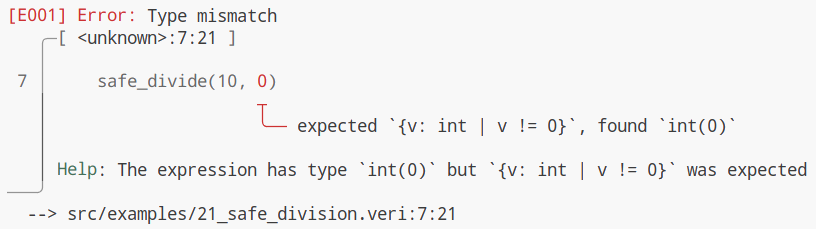
\includegraphics[scale=0.5]{figures/ariadne_error_message.png}
  \end{center}
  \caption{Example of a type error output formatted using the \texttt{ariadne} library.}
  \label{fig:type-error-message}
\end{figure}

\section{Middle end}\label{sec:middle-end}

\subsection{Typed Intermediate Representation (TIR)}

The TIR is a typed SSA (Static Single Assignment) intermediate representation. Each function is a control-flow graph of basic blocks; each block contains a sequence of three-address instructions followed by a terminator (jump, conditional branch, or return). Every instruction carries type annotations from the source-level type checker, and every virtual register is defined exactly once.

The choice of SSA was motivated by three properties: liveness analysis (required for register allocation) is straightforward, the one-definition property makes type annotations unambiguous, and phi nodes provide natural points for refinement type joining. At control-flow merge points, phi nodes select between values from different predecessor blocks.

A key extension beyond standard SSA is \textit{existential constraints on phi nodes}. Each phi node may carry an optional existential constraint of the form $\exists v.\; \mathtt{int}(v) \;\mathbf{where}\; \varphi(v)$, which encodes that the phi's value satisfies predicate $\varphi$ without fixing a concrete value. For loop induction variables, this captures the loop bounds: $\exists v.\; \mathtt{int}(v) \;\mathbf{where}\; (v \ge \mathit{start} \wedge v < \mathit{end})$. For mutable variables with refined types, it preserves the refinement predicate across iterations. This mechanism avoids the information loss that would occur if phi nodes were simply widened to the base type.

\subsubsection{Representative instruction forms}

TIR is designed to sit close to both the typed source language and the DTAL backend. The core forms relevant to the compilation pipeline are summarised in Figure~\ref{fig:tir-syntax}.

In concrete terms, a TIR function stores its parameters, pre/postconditions, and a map of basic blocks; each block contains entry phi nodes, ordinary instructions, a terminator, and an entry register state. This makes the representation explicit enough for code generation to be largely structural, while still retaining the source-level type information needed for later verification.

\begin{figure}[H]
{\small
\[
\renewcommand{\arraystretch}{1.09}
\begin{array}{@{}r@{\ }c@{\ }l@{\hspace{1.2em}}p{0.25\textwidth}@{}}
  \rho & ::= &
  v
  & \textbf{(Virtual registers)} \\[2pt]
  p & ::= &
  \rho : \tau
  & \textbf{(Typed parameters)} \\[2pt]
  \phi & ::= &
  \rho := \textsf{phi}\; \overrightarrow{(L,\rho)} : \tau\; \optclause{\textsf{where } C}
  & \textbf{(Phi nodes)} \\[4pt]
  I & ::= &
  \parbox[t]{0.66\textwidth}{
    $\rho := n : \tau \,|\, \rho := \rho' : \tau \,|\, \rho := \rho_1\; \textsf{op}\; \rho_2 : \tau \,|\, {}$\\
    $\rho := \textsf{unop}\; \rho' : \tau \,|\, \rho := \textsf{load}\; \rho_b[\rho_i] : \tau\; \textsf{where } C \,|\, {}$\\
    $\textsf{store}\; \rho_b[\rho_i] := \rho_s\; \textsf{where } C \,|\, {}$\\
    $\optclause{\rho :=}\; \textsf{call}\; f(\overrightarrow{\rho}) : \tau \,|\, \textsf{assume } C \,|\, \textsf{assert } C$
  }
  & \textbf{(Instructions)} \\[4pt]
  K & ::= &
  \parbox[t]{0.66\textwidth}{
    $\textsf{jump } L \,|\, \textsf{branch } \rho\; L_t\; L_f\; \textsf{where } C_t, C_f \,|\, \textsf{return}\; \optclause{\rho}$
  }
  & \textbf{(Terminators)} \\[4pt]
  B & ::= &
  L:\; \phi^*\; I^*\; K
  & \textbf{(Basic blocks)} \\[2pt]
  F & ::= &
  \textsf{fn } f(\overrightarrow{p}) \rightarrow \tau\; \optclause{\textsf{requires } C}\; \optclause{\textsf{ensures } C}\; \{B^*\}
  & \textbf{(Functions)}
\end{array}
\]
}
\caption{Veritas' core TIR syntax.}
\label{fig:tir-syntax}
\end{figure}

The grammar abstracts over the Rust data structures used in the implementation. Table~\ref{tab:tir-implementation-correspondence} gives the correspondence between the grammar and constructors in the implementation.

\begin{table}[H]
\centering
\footnotesize
\begin{tabular}{p{0.25\textwidth} p{0.7\textwidth}}
\hline
\textbf{Abstract TIR form} & \textbf{Implementation form} \\
\hline
$\rho := n : \tau$ & \texttt{LoadImm \{ dst, value, ty \}} \\
$\rho := \rho' : \tau$ & \texttt{Copy \{ dst, src, ty \}} \\
$\rho := \rho_1\;\textsf{op}\;\rho_2 : \tau$ & \texttt{BinOp \{ dst, op, lhs, rhs, ty \}} \\
$\rho := \textsf{unop}\;\rho' : \tau$ & \texttt{UnaryOp \{ dst, op, operand, ty \}} \\
$\rho := \textsf{load}\;\rho_b[\rho_i] : \tau\;\textsf{where } C$ & \texttt{ArrayLoad \{ dst, base, index, element\_ty, bounds\_constraint \}} \\
$\textsf{store}\;\rho_b[\rho_i] := \rho_s\;\textsf{where } C$ & \texttt{ArrayStore \{ base, index, value, bounds\_constraint \}} \\
$\optclause{\rho :=}\;\textsf{call}\;f(\overrightarrow{\rho}) : \tau$ & \texttt{Call \{ dst?, func, args, arg\_types, result\_ty \}} \\
$\textsf{assume } C$ & \texttt{AssumeConstraint \{ constraint \}} \\
$\textsf{assert } C$ & \texttt{AssertConstraint \{ constraint \}} \\
$\rho := \textsf{phi}\; \overrightarrow{(L,\rho)} : \tau$ & \texttt{PhiNode \{ dst, ty, incoming, existential\_constraint \}} \\
$\textsf{jump } L$ & \texttt{Jump \{ target \}} \\
$\textsf{branch } \rho\;L_t\;L_f$ & \texttt{Branch \{ cond, true\_target, false\_target, true\_constraint, false\_constraint \}} \\
$\textsf{return}\;\optclause{\rho}$ & \texttt{Return \{ value? \}} \\
\hline
\end{tabular}
\caption{Correspondence between the abstract TIR syntax and the implementation representation.}
\label{tab:tir-implementation-correspondence}
\end{table}

\subsection{Lowering from TAST to TIR}

The lowering pass translates the typed AST to TIR. A \texttt{LoweringContext} maintains a mapping from source-level variable names to virtual registers and tracks the current basic block under construction.

Lowering begins from the typed AST: each function arrives with typed parameters, a typed statement list, and an optional typed trailing expression. For each function, the lowerer:

\begin{enumerate}
  \item creates an entry block and initialises a fresh \texttt{LoweringContext};
  \item allocates a fresh virtual register for each parameter and records the corresponding source-variable binding;
  \item lowers the body statements in order, threading the context through the traversal;
  \item lowers the trailing expression, if present, to obtain the function's result register;
  \item closes the current block with a \texttt{Return} terminator;
  \item packages the accumulated basic blocks, phi nodes, entry states, and translated pre/postconditions into a \texttt{TirFunction}.
\end{enumerate}

\subsubsection{Syntax-directed translation}

Lowering is syntax-directed: each typed source construct becomes a small fragment of SSA code while threading the current variable-to-register map. Variable uses read the register currently associated with that source variable. A \texttt{let} binding lowers its right-hand side to a fresh virtual register and then extends the map with the new binding. For mutable variables, assignment lowers the right-hand side and updates the map so subsequent uses of the variable refer to the newly produced register; because TIR is in SSA form, the old register is never overwritten.

Expression forms lower similarly. Integer literals become \texttt{LoadImm}; arithmetic and comparisons become \texttt{BinOp} or \texttt{UnaryOp}; array reads and writes become \texttt{ArrayLoad} and \texttt{ArrayStore} with an explicit bounds constraint; and function calls become \texttt{Call} instructions carrying the argument registers, parameter-passing modes, and result type. Control-flow constructs introduce new basic blocks and terminators: an \texttt{if} expression lowers to a branch, two successor blocks, and a merge block with phi nodes for values and mutable variables that differ across the two paths; loops lower to entry/header/body/exit blocks with header phi nodes for loop-carried values.

\subsubsection{Control flow}

\textbf{Conditionals} are lowered in the standard SSA style: the condition branches to `then' and `else' blocks, which rejoin at a merge block. The only Veritas-specific detail is that each branch edge carries a logical constraint derived from the condition, so an \texttt{if x > 0} yields assumptions $x > 0$ and $\neg(x > 0)$ on the respective successors. Phi nodes are inserted only for variables whose assigned register differs between the two branches.

\textbf{For-loops} use the usual entry, header, body, and exit structure. The induction variable is represented by a header phi node with incoming values from the entry edge and the back-edge, and this phi carries an existential constraint recording the loop range $[\mathit{start}, \mathit{end})$. Mutable variables in scope also receive header phi nodes so that loop-carried values and loop-invariant values are explicit to the verifier.

\textbf{While-loops} are lowered similarly, except that the condition is re-evaluated in the header. Because the condition need not be a simple interval test, the lowerer cannot attach the same explicit range constraint used for \texttt{for} induction variables; verification instead relies on the translated branch condition and any programmer-supplied invariant.

\subsubsection{Constraint propagation}

Branch conditions are translated into the TIR's constraint language, which supports the same logical fragment as source-level specifications: linear arithmetic comparisons, logical connectives, bounded quantifiers, and array indexing. The crucial difference is that TIR constraints are expressed over virtual register names rather than source-level variables. This translation converts source-level expressions into \texttt{Constraint} values via a recursive traversal: comparisons map directly, logical operators produce constraint connectives, and quantifiers map to bounded quantified constraints.

The source-to-register shift is implemented by a variable-to-register substitution pass: constraints in the TAST refer to source-level variable names, but the TIR and DTAL operate on virtual register names. During lowering, the context maintains a substitution map from variable names to register names (e.g., \texttt{"lo"} $\mapsto$ \texttt{"v11"}), and all emitted constraints are rewritten accordingly. This ensures constraints remain valid through register allocation and DTAL verification.

Loop invariants are emitted in TIR as \texttt{AssertConstraint} instructions at the start of the loop body, after applying the variable-to-register substitution. During code generation, these become DTAL \texttt{assert} instructions. They are the TIR counterpart of invariant verification in the type checker: the type checker proves that the invariant holds, and the lower stages record it as an assertion for the verifier to re-check independently.

\section{Backend}\label{sec:backend}

\subsection{DTAL code generation}

The code generator translates the TIR forms of Figure~\ref{fig:tir-syntax} to DTAL, the dependently typed assembly language described in Section~\ref{sec:dtal-target-lang}. At this stage DTAL still uses virtual registers, but each basic block is annotated with a \textit{type state}: a mapping from registers to types together with the constraints known to hold at that program point. These annotations are the core of the type-preserving design, because they give the standalone verifier enough information to re-check the program without access to the source.

Most TIR instructions lower directly to DTAL. Phi nodes are implemented as parallel copies on predecessor edges, and array operations become address computations plus loads or stores with the relevant bounds constraints attached.

\subsection{Optimisation}

Optimisation runs on virtual-register DTAL before physical allocation. The implemented pipeline performs constant folding, local peephole rewrites, copy propagation, dead-code elimination, loop-invariant code motion, and a Veritas-specific load-operation fusion pass. The important design constraint is not the individual algorithms, but that they operate over a typed assembly representation rather than an untyped IR. Rewritten instructions must retain verifier-facing type annotations, and instructions with semantic or proof relevance---stores, calls, branches, stack operations, ownership events, and constraint assertions---are treated as effects rather than removable bookkeeping.

Two implementation details are specific to the later backend. First, constant folding may introduce immediate-form DTAL instructions such as \texttt{AddImm} and \texttt{CmpImm}, which have verifier rules and direct encoder cases. Second, load-operation fusion creates a \texttt{LoadOp} form to exploit x86-64 memory operands, but only where the original load has a single arithmetic use. Copy propagation is similarly conservative around physical-register materialisation moves, since those copies encode ABI-oriented structure needed by physical allocation.

\subsection{Register allocation}

Register allocation is implemented using standard liveness analysis followed by graph colouring. The default allocator is a Chaitin--Briggs style allocator over the 11 allocatable general-purpose x86-64 registers (excluding \texttt{rsp}, \texttt{rbp}, \texttt{rax}, \texttt{rdx}, and \texttt{r11}). Registers live across function calls are constrained to callee-saved registers (\texttt{rbx}, \texttt{r12}--\texttt{r15}), reflecting the calling convention. 

\subsection{Physical allocation}\label{sec:physalloc}

The register allocator produces a mapping from virtual to physical registers; the \textit{physical allocation pass} applies this mapping to produce a DTAL program that uses only physical registers. This is the central transformation in the default pipeline, and it is \textit{untrusted}---its output is verified by the DTAL verifier before code generation proceeds.

DTAL defines 16 physical registers: \texttt{r0}--\texttt{r12} (general purpose), \texttt{sp} (stack pointer), \texttt{fp} (frame pointer), and \texttt{lr} (link register / return value). These map directly to x86-64 registers:

\begin{table}[h]
\centering
\small
\begin{tabular}{l l l l}
\hline
\textbf{DTAL} & \textbf{x86-64} & \textbf{Role} & \textbf{Saved by} \\
\hline
\texttt{r0}--\texttt{r5} & \texttt{rdi}, \texttt{rsi}, \texttt{rdx}, \texttt{rcx}, \texttt{r8}, \texttt{r9} & Arguments 1--6 & Caller \\
\texttt{r6}--\texttt{r7} & \texttt{r10}, \texttt{r11} & Scratch & Caller \\
\texttt{r8}--\texttt{r12} & \texttt{rbx}, \texttt{r12}--\texttt{r15} & General & Callee \\
\texttt{lr} & \texttt{rax} & Return value & Caller \\
\texttt{sp} & \texttt{rsp} & Stack pointer & --- \\
\texttt{fp} & \texttt{rbp} & Frame pointer & --- \\
\hline
\end{tabular}
\caption{DTAL physical register mapping to x86-64.}
\label{tab:regmap}
\end{table}

Beyond simple register renaming, the physical allocation pass performs several x86-specific transformations:

\begin{itemize}
  \item \textbf{Function prologues and epilogues}: emits explicit \texttt{Prologue} and \texttt{Epilogue} instructions that push/pop callee-saved registers and allocate a 16-byte-aligned stack frame.
  \item \textbf{Division expansion}: a single virtual \texttt{div} instruction is expanded to the x86-64 sequence 
\begin{center}
\begin{minipage}{0.35\textwidth}
\centering
\begin{minted}[escapeinside=||]{text}
mov rax, lhs
cqo
idiv rhs
mov dst, rax|\footnotemark|
\end{minted}
\end{minipage}
\end{center}
\footnotetext{or \texttt{rdx} for modulo.}
since \texttt{idiv} requires its operands in the \texttt{rdx:rax} pair.
  \item \textbf{Caller-saved register management}: at each call site, caller-saved registers that are live across the call are spilled to the stack before argument setup and restored after the call returns using explicit \texttt{SpillStore} and \texttt{SpillLoad} instructions, with the verifier checking spill-slot type consistency.
  \item \textbf{Parameter move cycle resolution}: when function parameters must be shuffled between registers (e.g., parameter~0 in \texttt{rdi} must move to \texttt{rsi}, while parameter~1 in \texttt{rsi} must move to \texttt{rcx}), the pass detects cycles and breaks them using \texttt{r11} as a scratch register.
  \item \textbf{Constraint remapping}: all type constraints are rewritten from virtual register names (\texttt{v3}) to physical register names (\texttt{r0}), so the verifier can check the physical program.
\end{itemize}

\subsection{Direct encoding}\label{sec:direct-encoding}

The \textit{direct encoder} translates physically-allocated DTAL to x86-64 machine code. Because the physical allocation pass has already performed all x86-specific expansions (division, calling convention, prologues), the encoder is a near-trivial 1:1 mapping: each DTAL instruction maps to exactly one x86-64 instruction (or a short fixed sequence for prologues and epilogues). The entire module is 309 lines in the current implementation.

This simplicity is deliberate and architecturally significant. Initially, I implemented a monolithic x86-64 lowering pass that performed register allocation, instruction selection, and encoding in a single trusted step. By splitting this into an untrusted physical allocation pass (verified by the DTAL verifier) and a small encoder, most register-allocation and instruction-selection logic is moved outside the trusted path. The encoder still remains trusted, so its small size is an auditability argument rather than a proof of correctness.

\subsection{Binary encoding and ELF generation}

The direct encoder emits x86-64 machine code from physical DTAL, using a two-pass scheme to resolve label offsets. The resulting byte stream is then wrapped in a minimal ELF executable with entry point \texttt{main}; for the Linux target this is an ELF64 binary, while the bare-metal target uses a separate Multiboot-compatible layout described below.

\section{Independent verifier}\label{sec:verifier}

A key contribution of the type-preserving architecture is that the DTAL output can be verified independently of the compiler. The verifier re-checks the DTAL program from scratch, using only the type annotations embedded in the assembly. It follows the derivation-based verification approach of Xi and Harper~\cite{Xi2001DTAL}: types are \textit{re-derived} from instruction semantics, not trusted from compiler annotations.

\subsection{Verification algorithm}

The verifier processes each function independently. For each basic block, it:

\begin{enumerate}
  \item Initialises the type state from the block's declared entry state (register types and constraints).
  \item Symbolically executes each instruction, \textit{re-deriving} the result type from the operand types according to the instruction's semantics.
  \item At each constraint assertion (\texttt{.assert}), invokes its own SMT oracle to verify that the constraint follows from the current type state.
  \item At block exits (jumps, branches, returns), performs \textit{state coercion}: verifies that the computed exit state is compatible with the declared entry state of each successor block.
\end{enumerate}

The re-derivation in step 2 is central to the untrusted-compiler model. For example, \texttt{mov rd, 5} always derives $\texttt{rd} : \mathtt{int}(5)$ from the immediate value, regardless of any annotation the compiler may have emitted. Similarly, \texttt{add rd, r1, r2} derives $\texttt{rd} : \mathtt{int}(\texttt{r1} + \texttt{r2})$ using symbolic index expression algebra. The compiler's annotations serve only as a cross-check; if the re-derived type conflicts with the annotation, the verifier reports an error.

\subsection{State coercion at control-flow edges}

State coercion is how the verifier checks compatibility across block boundaries. When block A jumps to block B, it must show that A's exit state is a subtype of B's declared entry state. This reduces to two checks:

\begin{itemize}
  \item \textbf{Register type subtyping}: for each register in B's entry state, A's exit type must be a subtype. The subtyping relation is constraint-aware: $\mathtt{int}(n) <: \mathtt{int}$ always holds, and $\mathtt{int}(n) <: \exists v.\; \mathtt{int}(v) \;\mathbf{where}\; \varphi(v)$ holds if $\varphi(n)$ is provable from A's constraints.
  \item \textbf{Constraint entailment}: every constraint declared in B's entry state must be provable from A's exit constraints.
\end{itemize}

For conditional branches, the verifier first refines the exit state on each edge. For example, \texttt{cmp r1, r2} followed by \texttt{jl target} contributes $\texttt{r1} < \texttt{r2}$ on the taken edge and $\texttt{r1} \ge \texttt{r2}$ on the fall-through edge before coercion is checked against the respective successor states.

\subsection{Array bounds verification}

Array loads and stores are the most critical instructions for the verifier. For each \texttt{load rd, [base + offset]}:

\begin{enumerate}
  \item The verifier checks that \texttt{base} has an array type $[\tau; N]$.
  \item It constructs the bounds obligation $0 \le \texttt{offset} < N$.
  \item It attempts to prove this obligation, first via fast syntactic checks (e.g., is the constraint already in the context?), then via the SMT oracle.
  \item If the proof succeeds, it derives the element type $\tau$ for \texttt{rd} and emits a \textit{select axiom}: $\texttt{rd} = \mathit{arr}[\texttt{offset}]$, linking the loaded value to the array's logical representation.
\end{enumerate}

\noindent Stores additionally emit two axioms: 
\begin{tcolorbox}[colback=blue!5!white,colframe=blue!75!black]
  \paragraph{Write axiom.} $\mathit{arr}_{\mathit{new}}[\texttt{offset}] = \texttt{value}$ \\

  \paragraph{Frame axiom.} $\forall k \ne \texttt{offset}.\; \mathit{arr}_{\mathit{new}}[k] = \mathit{arr}_{\mathit{old}}[k]$
\end{tcolorbox}
The array is tracked with a version number that increments on each store, ensuring that the SMT solver can distinguish array states before and after mutations.

\subsection{Interprocedural contract verification}

When the verifier encounters a \texttt{call} instruction, it performs three checks:

\begin{enumerate}
  \item \textbf{Precondition}: the callee's precondition, with formal parameters substituted for actual argument registers, must be provable from the caller's current constraints.
  \item \textbf{Return type}: the callee's declared return type is assigned to the destination register.
  \item \textbf{Postcondition}: the callee's postcondition (similarly substituted) is added to the caller's constraint set for use by subsequent instructions.
\end{enumerate}

This enables modular verification: each function is checked in isolation, relying on contracts rather than inlining.

\subsection{SMT oracle}

The verifier uses its own Z3 instance, completely independent of the one used during compilation. The translation follows the same proof-by-refutation approach as the compiler's oracle (Section~\ref{sec:smt-oracle}): assert the context, assert the negated goal, and check for unsatisfiability.

To improve performance, constraint provability uses a two-tier approach. A fast syntactic check handles common cases (constraint already in context, simple entailment patterns) in $O(n)$ where $n$ is the context size. The SMT solver is invoked only when the syntactic check is inconclusive. This is important because the verifier issues many more queries than the compiler---one per instruction rather than one per subtyping check.

\subsection{Verification after register allocation}

% The compiler supports two pipeline modes. The \textit{legacy pipeline} (\texttt{--legacy-pipeline}) verifies the virtual-register DTAL and then trusts the x86-64 lowering (register allocation, instruction selection, encoding). The \textit{physical pipeline} (the default) defers verification until \textit{after} register allocation has mapped virtual registers to physical x86-64 registers. In the physical pipeline, 
The verifier checks the physically-allocated DTAL, meaning that register allocation, spill insertion, and calling-convention lowering are all \textit{untrusted} for the checked safety policy: bugs in these passes manifest as a type derivation mismatch or unprovable constraint in the verified output.

This is a deliberate architectural choice. Register allocation is one of the most error-prone compiler passes (it involves liveness analysis, graph colouring, spill heuristics, and calling-convention details), and verifying its output rather than trusting it substantially reduces the trusted computing base, evident in the implementation of the direct encoder (Section~\ref{sec:direct-encoding}).

% \subsection{Trust model}
%
% The trust model and TCB reduction phases are described in Section~\ref{sec:design-decisions}. The verification architecture places the trust boundary between the physical DTAL verifier and the direct encoder: the compiler frontend, middle end, backend, and register allocator are outside the trusted path for the checked DTAL safety policy. The verifier does not prove full semantic preservation, so a type-consistent compiler bug could still compute the wrong value while passing the safety check.

\section{Runtime}\label{sec:runtime}

The compiler provides a small set of runtime intrinsics that are linked into every executable. These are implemented as hand-assembled x86-64 machine code totalling approximately 210 bytes, prepended to the user's compiled code in the ELF output.

Five intrinsics are provided:

\begin{itemize}
  \item \texttt{print\_int(n: int)}: converts a signed 64-bit integer to its decimal string representation and writes it to stdout followed by a newline, using the Linux \texttt{write} syscall.
  \item \texttt{print\_char(c: int)}: writes a single byte to stdout.
  \item \texttt{read\_int() -> int}: reads a decimal integer from stdin using the Linux \texttt{read} syscall, handling an optional leading minus sign.
  \item \texttt{port\_in(port: int) -> int}: reads a byte from an x86 I/O port using the \texttt{in} instruction.
  \item \texttt{port\_out(port: int, val: int)}: writes a byte to an x86 I/O port using the \texttt{out} instruction.
\end{itemize}

The first three intrinsics use Linux syscalls and are available only when compiling for the Linux target. The port I/O intrinsics use hardware instructions directly and are available on both Linux and bare-metal targets. The type checker enforces this distinction: a bare-metal program that calls \texttt{print\_int} is rejected at compile time rather than failing at runtime.

All intrinsics follow the System~V AMD64 calling convention (first argument in \texttt{rdi}, return value in \texttt{rax}), so they are callable from compiled Veritas code without any marshalling. Because the runtime is hand-assembled and part of the trusted computing base, its correctness is assumed on the basis of its small size, tests, and inspection rather than established by the DTAL verifier.

\section{Bare-metal target}\label{sec:unikernel}
% TODO: elaborate more on implementation; highlight as extension and purpose to support I/O functionality

The \texttt{--target-bare-metal} flag in the Veritas CLI produces a Multiboot-compliant ELF32 that can boot directly on x86-64 hardware or QEMU\footnote{QEMU is an open-source machine emulator and virtualiser: \url{https://www.qemu.org/}.} without an operating system. This removes the host operating-system kernel from the normal execution path for this target, replacing it with a small trusted bootstrap and runtime. The bootstrap, runtime intrinsics, hardware model, and QEMU behaviour remain outside the DTAL verifier's guarantee.

\subsection{Bootstrap}

The bare-metal binary begins with a bootstrap blob of approximately 200 bytes that performs the transition from the Multiboot entry point (32-bit protected mode) to 64-bit long mode:

\begin{enumerate}
  \item A Multiboot header allows GRUB or QEMU's \texttt{-kernel} flag to load the binary.
  \item The bootstrap sets up a minimal page table (identity-mapping the first 8\,MB using four 2\,MB huge pages), enables PAE and long mode via the appropriate control register writes, and performs a far jump into 64-bit code.
  \item A GDT (Global Descriptor Table) with 64-bit code and data segments is loaded.
  \item The stack pointer is set to a fixed address (\texttt{0x200000}) and \texttt{main} is called.
  \item After \texttt{main} returns, the bootstrap enters a \texttt{hlt} loop.
\end{enumerate}

The bootstrap is hand-assembled and part of the trusted computing base; at $\sim$200 bytes it is intended to remain small enough for line-by-line audit.

\subsection{DTAL-checked serial driver}

To demonstrate DTAL-checked code generation for bare-metal I/O, the project includes a serial driver written entirely in Veritas. The driver programs the UART 16550 controller (the standard PC serial port at I/O base \texttt{0x3F8}) using the \texttt{port\_in} and \texttt{port\_out} intrinsics:

\begin{itemize}
  \item \texttt{serial\_init()} configures the baud rate (38400), line format (8N1), and FIFO.
  \item \texttt{serial\_write(c: int)} spins on the Line Status Register until the transmit buffer is empty, then writes a byte to the data register.
  \item \texttt{serial\_print\_int(n: int)} recursively prints a signed integer to the serial port.
\end{itemize}

The entire driver is type-checked and compiled through the verified DTAL pipeline. When compiled with \texttt{--target-bare-metal --verify -o serial}, the resulting binary boots in QEMU and outputs to the serial console:

\begin{verbatim}
  qemu-system-x86_64 -kernel serial -serial stdio
\end{verbatim}

This demonstrates the project's long-term direction: a bare-metal Veritas target in which application code and simple drivers are checked as DTAL before encoding, while a small trusted bootstrap and runtime replace the host operating-system kernel. Figure~\ref{fig:unikernel-arch} illustrates the architecture of a bare-metal Veritas binary.

\begin{figure}[H]
  \centering
  \begin{tikzpicture}[
      font=\small,
      scale=0.8
    ]
    % Hardware
    \draw[thick] (0,11.0) rectangle (13.4,12.35);
    \node[font=\small\bfseries] at (6.7,11.88) {Hardware (x86-64)};
    \node[font=\scriptsize] at (6.7,11.35) {CPU \hspace{0.4cm} RAM \hspace{0.4cm} Serial (COM1 @ 0x3F8) \hspace{0.4cm} VGA \hspace{0.4cm} Disk \hspace{0.4cm} NIC};

    \draw[-Latex, thick] (6.7,11.0) -- (6.7,10.3);
    \node[font=\scriptsize, align=center, fill=white, inner sep=1pt] at (9.0,10.65) {port I/O / memory-mapped I/O};

    % Outer bare-metal binary
    \draw[thick] (0,0.8) rectangle (13.4,10.2);
    \node[font=\small\bfseries] at (6.7,9.8) {Bare-metal Veritas ELF};

    % Bootstrap
    \draw[thick] (0.7,8.2) rectangle (12.7,9.3);
    \node[anchor=west] at (1.0,8.82) {Bootstrap};
    \node[anchor=west, font=\scriptsize] at (1.0,8.45) {Multiboot header $\rightarrow$ 32$\rightarrow$64 bit $\rightarrow$ PAE/paging $\rightarrow$ GDT $\rightarrow$ \texttt{main}};

    \draw[-Latex, thick] (6.7,8.2) -- (6.7,7.6);

    % Runtime intrinsics
    \draw[thick] (0.7,5.0) rectangle (12.7,7.5);
    \node[anchor=west] at (1.0,7.1) {Runtime Intrinsics};
    \node[anchor=west, font=\scriptsize] at (1.0,6.6) {\texttt{port\_in(port) -> int}};
    \node[anchor=west, font=\scriptsize] at (7.2,6.6) {\texttt{port\_out(port, val)}};

    \draw[thick] (1.15,5.23) rectangle (5.5,6.29);
    \node[anchor=west, font=\scriptsize] at (1.35,6.12) {\texttt{mov dx, di}};
    \node[anchor=west, font=\scriptsize] at (1.35,5.92) {\texttt{in  al, dx}};
    \node[anchor=west, font=\scriptsize] at (1.35,5.72) {\texttt{movzx rax, al}};
    \node[anchor=west, font=\scriptsize] at (1.35,5.52) {\texttt{ret}};

    \draw[thick] (7.2,5.23) rectangle (11.95,6.29);
    \node[anchor=west, font=\scriptsize] at (7.4,6.12) {\texttt{mov dx, di}};
    \node[anchor=west, font=\scriptsize] at (7.4,5.92) {\texttt{mov al, sil}};
    \node[anchor=west, font=\scriptsize] at (7.4,5.72) {\texttt{out dx, al}};
    \node[anchor=west, font=\scriptsize] at (7.4,5.52) {\texttt{ret}};

    \draw[-Latex, thick] (6.7,5.0) -- (6.7,4.45);

    % DTAL-checked application code
    \draw[thick] (0.7,1.5) rectangle (12.7,4.35);
    \node[anchor=west] at (1.0,4.0) {DTAL-checked Application Code};

    \draw[thick] (1.15,2.15) rectangle (12.0,3.7);
    \node[anchor=west, font=\scriptsize\bfseries] at (1.4,3.45) {\texttt{serial\_driver.veri}};
    \node[anchor=west, font=\scriptsize] at (1.4,3.08) {\texttt{serial\_init()}: configure UART 16550 (8N1, 38400 baud, FIFO enabled)};
    \node[anchor=west, font=\scriptsize] at (1.4,2.73) {\texttt{serial\_write(c)}: poll LSR bit 5, then \texttt{port\_out(COM1, c)}};
    \node[anchor=west, font=\scriptsize] at (1.4,2.38) {\texttt{main()}: initialise serial, print integers, halt};
  \end{tikzpicture}
  \captionsetup{
    aboveskip=4pt,
    belowskip=-8pt
  }
  \caption{Architecture of a bare-metal Veritas binary. The binary contains a trusted Multiboot bootstrap, a small set of hand-assembled runtime intrinsics, and application code checked through the DTAL pipeline.}
  \label{fig:unikernel-arch}
\end{figure}

\section{Borrowing and ownership extension}\label{sec:ownership-extension}

The core refinement type system does not by itself control aliasing. This is a serious limitation for a systems-language fragment: mutation through one name can invalidate facts assumed through another name, and unrestricted references make it unclear which part of the program owns a mutable object. Veritas adds a Rust-inspired ownership and borrowing discipline: the source checker rejects obvious aliasing errors, while TIR and DTAL preserve ownership events explicitly so that the final low-level verifier can check that the backend has not introduced an illegal move, duplicated owner, or conflicting borrow.

% \subsection{Source-language design}

% The source extension adds shared references, mutable references, borrow expressions, and dereference expressions. 
The supported fragment is lexical and first-order: borrows are tied to source bindings, block exit ends borrows introduced in that block, and references are not stored in aggregates or returned from functions. This keeps the model compatible with the rest of the Veritas type checker while still supporting the common systems-language patterns needed by the feature suite: shared array reads, mutable array updates, scalar dereference, and reference parameters.

\begin{table}[H]
\centering
\small
\begin{tabular}{p{0.28\textwidth} p{0.30\textwidth} p{0.32\textwidth}}
\hline
\textbf{Source form} & \textbf{Meaning} & \textbf{Main check} \\
\hline
\texttt{\&T} & Shared reference type & Read-only alias to a value of type \texttt{T}. \\
\texttt{\&mut T} & Mutable reference type & Unique mutable alias to a value of type \texttt{T}. \\
\texttt{\&x} & Shared borrow & Rejected if \texttt{x} is currently mutably borrowed. \\
\texttt{\&mut x} & Mutable borrow & Rejected unless \texttt{x} is mutable and has no live borrows. \\
\texttt{*r} & Scalar dereference & Requires \texttt{r} to have reference type; assignment through \texttt{*r} requires \texttt{\&mut}. \\
\texttt{r[i]} & Array-reference indexing & Uses the referenced array and proves the usual bounds obligation. \\
\hline
\end{tabular}
\caption{Source-level ownership and borrowing forms.}
\label{tab:source-ownership-forms}
\end{table}

% For example, a mutable scalar borrow is written directly in the source language:

\begin{figure}[H]
\begin{center}
\begin{cminted}{rust}
fn main() -> int {
    let mut x: int = 0;
    let mx: &mut int = &mut x;
    *mx = 9;
    *mx
}
\end{cminted}
\end{center}
\caption{A mutable scalar borrow in the Veritas source language.}
\label{fig:source-mutable-borrow}
\end{figure}

% \subsection{Frontend implementation}

Borrowing is implemented as an extension of the ordinary bidirectional type checker. In addition to the contexts $(\phi, \Gamma, \Delta \Sigma_F)$, the concrete \texttt{TypingContext} records ownership metadata:

\begin{table}[H]
\centering
\small
\begin{tabular}{p{0.30\textwidth} p{0.58\textwidth}}
\hline
\textbf{Context component} & \textbf{Role} \\
\hline
\texttt{moved\_bindings} & Bindings whose ownership has been transferred and cannot be used again until reinitialised. \\
\texttt{active\_borrows} & For each owner, records live shared-borrow counts and whether a mutable borrow is live. \\
\texttt{borrow\_bindings} & Maps reference bindings back to the owner they borrow from and the borrow kind. \\
\texttt{borrow\_scopes} & Stack of lexical scopes used to release borrows at block exit. \\
\hline
\end{tabular}
\caption{Ownership-specific state maintained by the frontend typing context.}
\label{tab:frontend-ownership-context}
\end{table}

Creating \texttt{\&x} increments the shared-borrow count for \texttt{x}; creating \texttt{\&mut x} requires no live shared or mutable borrow. Assignments, shadowing, moves, and function calls consult the same metadata, so the checker rejects mutating a shared-borrowed owner, moving a borrowed owner, creating a shared borrow while a mutable borrow is live, and creating two simultaneous mutable borrows. These checks are integrated into \texttt{check\_stmt} and \texttt{synth\_expr}, which means the typed AST records both the ordinary type of an expression and the borrow/move behaviour needed by lowering.

% \subsection{TIR representation}

Once the frontend accepts a program, ownership behaviour is made explicit in TIR. This is important because later compiler stages should not need to reconstruct ownership events from source syntax: the verifier-facing pipeline receives first-class operations for moves, drops, borrow creation, and borrow termination.

\begin{table}[H]
\centering
\small
\begin{tabular}{p{0.34\textwidth} p{0.52\textwidth}}
\hline
\textbf{TIR form} & \textbf{Purpose} \\
\hline
\texttt{MoveOwned \{ dst, src, ty \}} & Transfers ownership from \texttt{src} to \texttt{dst}; the old owner cannot be used as owned afterwards. \\
\texttt{DropOwned \{ src, ty \}} & Ends ownership of a value at a known program point. \\
\texttt{BorrowShared \{ dst, src, ty \}} & Creates a shared borrow of \texttt{src}. \\
\texttt{BorrowMut \{ dst, src, ty \}} & Creates a unique mutable borrow of \texttt{src}. \\
\texttt{BorrowEnd \{ src, ty \}} & Ends the borrow held in \texttt{src}. \\
\texttt{Call \{ ..., arg\_kinds, ownership, ... \}} & Records whether parameters are plain values, owned values, shared borrows, or mutable borrows. \\
\hline
\end{tabular}
\caption{Ownership-aware TIR instructions and metadata.}
\label{tab:tir-ownership-forms}
\end{table}

Scalar references require one additional implementation device. Arrays already have a memory representation in TIR and DTAL, so borrowing an array can target the array directly. A scalar value, however, must be made addressable before it can be borrowed. The lowerer therefore uses a hidden one-element cell for scalar references: it allocates a size-1 cell, stores the scalar value into it, borrows the cell, and lowers dereference to an ordinary load or store through that cell. This allows scalar references to reuse the same array load/store and bounds-checking machinery rather than introducing a separate pointer memory model.

% \subsection{DTAL representation}

The ownership-aware TIR forms lower to explicit DTAL instructions. The extension also adds shared and mutable reference types, written $\&\tau$ and $\&\textsf{mut } \tau$, which classify registers holding borrow capabilities. These instructions do not perform computation in the ordinary arithmetic sense; they update the verifier's ownership state and make aliasing behaviour visible in the low-level artifact.

\begin{table}[H]
\centering
\small
\begin{tabular}{p{0.32\textwidth} p{0.54\textwidth}}
\hline
\textbf{DTAL form} & \textbf{Verifier-visible meaning} \\
\hline
\texttt{move\_owned rd, rs : T} & Transfers ownership from \texttt{rs} to \texttt{rd}. \\
\texttt{drop\_owned rs : T} & Consumes the owned value in \texttt{rs}. \\
\texttt{alias\_borrow rd, rs : \&T} & Creates a shared borrow of the object held by \texttt{rs}. \\
\texttt{borrow\_mut rd, rs : \&mut T} & Creates a mutable borrow of the object held by \texttt{rs}. \\
\texttt{borrow\_end rs : \&T} or \texttt{\&mut T} & Ends the borrow held in \texttt{rs}. \\
\hline
\end{tabular}
\caption{Ownership and borrowing instructions added to V-DTAL.}
\label{tab:dtal-ownership-forms}
\end{table}

A representative fragment after lowering a shared borrow has the following shape:

\begin{figure}[H]
\begin{center}
\begin{cminted}{text}
alias_borrow v3, v1    : &[int(7); 1]
load v5, [v3 + v4]     : int
borrow_end v3          : &[int(7); 1]
\end{cminted}
\end{center}
\caption{Verifier-visible DTAL operations for a shared array borrow.}
\label{fig:dtal-shared-borrow}
\end{figure}

The important property is that the backend cannot silently erase the source-level ownership discipline. If it emits a second mutable borrow, moves an owner while a borrow is live, or fails to end a borrow on one control-flow path, the final DTAL program is inconsistent with the verifier's ownership state and is rejected.

% \subsection{Verifier support}

The independent verifier extends its ordinary register-and-constraint state with ownership metadata. It tracks which registers currently hold owned values, assigns object identities to owned values, records which registers hold shared or mutable borrows of each object, and records consumed registers. The instruction checker then enforces the capability discipline shown in Table~\ref{tab:verifier-ownership-rules}.

\begin{table}[H]
\centering
\small
\begin{tabular}{p{0.32\textwidth} p{0.54\textwidth}}
\hline
\textbf{Rule} & \textbf{Effect} \\
\hline
Move availability & \texttt{move\_owned} requires the source register to hold a live owned object. \\
Borrow exclusion & \texttt{borrow\_mut} is rejected if the object has any live shared or mutable borrow. \\
Shared borrow compatibility & \texttt{alias\_borrow} is allowed for shared borrows but rejected while a mutable borrow is live. \\
Borrowed-owner protection & \texttt{move\_owned} and \texttt{drop\_owned} are rejected while the object is borrowed. \\
Borrow termination & \texttt{borrow\_end} requires the register to hold a live borrow and releases it from the object state. \\
Control-flow joins & Join states must agree on live ownership and borrow information; one-sided borrow endings are rejected. \\
\hline
\end{tabular}
\caption{Ownership rules enforced by the DTAL verifier.}
\label{tab:verifier-ownership-rules}
\end{table}

This state is preserved through register allocation, spills, reloads, stack operations, and physical register shuffles. As a result, the checked property is stronger than source-level borrow checker acceptance: the post-register-allocation DTAL program must still exhibit a consistent ownership and borrowing discipline immediately before direct machine-code encoding.
% ``the source borrow checker once accepted the program'': the post-register-allocation DTAL program must still exhibit a consistent ownership and borrowing discipline immediately before direct machine-code encoding.

% \subsection{Scope and limitations}
%
% The implementation is intentionally not a full Rust borrow checker. It does not infer non-lexical lifetimes, support returned references, support reborrowing, store references in aggregate values, or borrow substructure such as \texttt{\&arr[i]}. These restrictions are design trade-offs rather than parser accidents: they keep the source checker, TIR lowering, DTAL instruction set, and verifier state small enough to support the dissertation's main trust argument. Within this scoped fragment, ownership and borrowing are preserved through the full pipeline rather than remaining a source-only check.



% \section{Worked example: binary search}\label{sec:worked-example}
% %
% The preceding sections describe each pipeline stage in isolation. This section demonstrates the full pipeline by tracing a \texttt{binary\_search} program, from source to verified DTAL. Binary search features most of the verification and constraint features of Veritas: quantified preconditions, refinement types, loop invariants, array bounds proofs, existential types, branch constraint refinement, and symbolic arithmetic.
%
% \subsection{Source language}
% %
% The source program searches a sorted 10-element array for a target value, returning its index or $-1$ if not found:
% %
% \begin{quote}
% \begin{verbatim}
% fn binary_search(arr: [int; 10], target: int) -> int
%     requires forall i in 0..9 { arr[i] <= arr[i + 1] }
% {
%     let mut lo: {v: int | v >= 0} = 0;
%     let mut hi: int = 9;
%     let mut result: int = -1;
%
%     for iter in 0..20
%         invariant lo >= 0 && hi < 10
%     {
%         if lo <= hi {
%             let mid: int = lo + (hi - lo) / 2;
%             let val: int = arr[mid];
%             if val == target {
%                 result = mid;
%                 lo = hi + 1;
%             } else {
%                 if val < target {
%                     lo = mid + 1;
%                 } else {
%                     hi = mid - 1;
%                 }
%             }
%         } else {
%             let done: int = 0;
%         }
%     }
%
%     result
% }
% \end{verbatim}
% \end{quote}
% %
% Several features are worth highlighting:
% %
% \begin{itemize}
%   \item \texttt{requires forall i in 0..9 \{ arr[i] <= arr[i+1] \}} --- a quantified precondition asserting that the array is sorted in non-decreasing order. This is checked at every call site.
%   \item \texttt{\{v: int | v >= 0\}} --- a refinement type on \texttt{lo}, constraining it to be non-negative. This is the master type: every assignment to \texttt{lo} must satisfy it.
%   \item \texttt{invariant lo >= 0 \&\& hi < 10} --- a loop invariant that bounds both endpoints. The type checker verifies this holds initially and is preserved by the loop body.
%   \item \texttt{arr[mid]} --- the critical array access. The type checker must prove $0 \le \mathtt{mid} < 10$ from the invariant and branch conditions.
%   \item \texttt{for iter in 0..20} --- the loop uses a bounded iteration counter. Although Veritas also supports \texttt{while} loops, the bounded \texttt{for} loop is useful here because it yields an explicit induction-variable range in the generated SSA and DTAL.
% \end{itemize}
%
% \subsection{Frontend type checking}
% %
% The type checker discharges three key proof obligations for this function. All are reduced to SMT queries of the form: assert the current context $\phi$, assert $\lnot G$ (the negated goal), and check for unsatisfiability.
% %
% \subsubsection{Loop invariant: base case}
% %
% Before the loop begins, the context contains $\mathtt{lo} = 0$ (from the singleton type $\mathtt{int}(0)$) and $\mathtt{hi} = 9$ (from $\mathtt{int}(9)$). The invariant to verify is:
% \[
%   \mathtt{lo} \ge 0 \;\wedge\; \mathtt{hi} < 10
% \]
% Substituting the initial values gives $0 \ge 0 \wedge 9 < 10$, which is trivially satisfiable. The SMT oracle confirms this by showing that $\lnot(0 \ge 0 \wedge 9 < 10)$ is unsatisfiable.
% %
% \subsubsection{Loop invariant: inductive step}
% %
% At the end of the loop body, the type checker must prove that the invariant is preserved. The context at this point includes the assumed invariant ($\mathtt{lo} \ge 0 \wedge \mathtt{hi} < 10$) plus the branch conditions taken during the iteration. In each branch:
% \begin{itemize}
%   \item \texttt{val == target}: \texttt{lo} is set to \texttt{hi + 1}. Since $\mathtt{hi} < 10$, we have $\mathtt{lo} = \mathtt{hi} + 1 \ge 1 \ge 0$, and \texttt{hi} is unchanged.
%   \item \texttt{val < target}: \texttt{lo} is set to \texttt{mid + 1}. Since $\mathtt{mid} \ge 0$ (from $\mathtt{lo} \ge 0$ and the midpoint formula), $\mathtt{lo} \ge 1 \ge 0$, and \texttt{hi} is unchanged.
%   \item Otherwise: \texttt{hi} is set to \texttt{mid - 1}. Since $\mathtt{mid} < 10$ (from $\mathtt{hi} < 10$ and the midpoint formula), $\mathtt{hi} < 10$, and \texttt{lo} is unchanged.
% \end{itemize}
% %
% At the join point, the context-joining operation computes the least upper bound across all branches, and the SMT oracle verifies the invariant holds under the joined context.
% %
% \subsubsection{Array bounds for \texttt{arr[mid]}}
% %
% The array access \texttt{arr[mid]} occurs inside the branch guarded by \texttt{lo <= hi}. At this point the context contains:
% \[
%   \phi = \{\, \mathtt{lo} \ge 0, \;\; \mathtt{hi} < 10, \;\; \mathtt{lo} \le \mathtt{hi}, \;\; \mathtt{mid} = \mathtt{lo} + (\mathtt{hi} - \mathtt{lo}) / 2 \,\}
% \]
% The proof obligation is $0 \le \mathtt{mid} < 10$. From the context:
% \begin{itemize}
%   \item $\mathtt{mid} \ge \mathtt{lo} \ge 0$ (since $(\mathtt{hi} - \mathtt{lo})/2 \ge 0$ when $\mathtt{lo} \le \mathtt{hi}$)
%   \item $\mathtt{mid} \le \mathtt{hi} < 10$ (since $\mathtt{mid} = \mathtt{lo} + (\mathtt{hi} - \mathtt{lo})/2 \le \mathtt{hi}$)
% \end{itemize}
% The SMT oracle asserts $\phi \wedge \lnot(0 \le \mathtt{mid} \wedge \mathtt{mid} < 10)$ and obtains UNSAT, confirming the bounds proof.
%
% \subsection{Lowering to TIR (SSA)}
% %
% The lowering pass translates the function into a control-flow graph of 13 basic blocks. Figure~\ref{fig:bs-cfg} shows the structure, with blocks grouped by their role in the algorithm.
% %
% \begin{figure}[H]
%   \centering
%   \begin{tikzpicture}[
%       scale=0.75, transform shape,
%       block/.style={rectangle, draw, thick, text centered,
%           minimum height=0.6cm, minimum width=0.9cm,
%           font=\small\ttfamily},
%       arrow/.style={-Stealth, thick},
%       lbl/.style={font=\scriptsize, text=black!60},
%       elbl/.style={font=\scriptsize, text=black!60, fill=white, inner sep=1pt}
%     ]
%     % Row 0: entry
%     \node[block] (bb0) at (0,0) {bb0};
%     \node[lbl, right=0.15cm of bb0] {entry};
%
%     % Row 1: loop header
%     \node[block] (bb1) at (0,-1.6) {bb1};
%     \node[lbl, left=0.15cm of bb1] {loop header};
%
%     % Row 2: body / exit
%     \node[block] (bb2) at (-2,-3.4) {bb2};
%     \node[lbl, left=0.15cm of bb2] {body};
%     \node[block] (bb3) at (3,-3.4) {bb3};
%     \node[lbl, right=0.15cm of bb3] {exit};
%
%     % Row 3: lo<=hi / lo>hi
%     \node[block] (bb4) at (-3.5,-5.2) {bb4};
%     \node[block] (bb5) at (0.5,-5.2) {bb5};
%
%     % Row 4: val==target / val!=target
%     \node[block] (bb7) at (-5,-7.0) {bb7};
%     \node[block] (bb8) at (-2,-7.0) {bb8};
%
%     % Row 5: join from == / val<target / val>=target
%     \node[block] (bb9) at (-5,-8.8) {bb9};
%     \node[block] (bb10) at (-3,-8.8) {bb10};
%     \node[block] (bb11) at (-1.7,-8.8) {bb11};
%
%     % Row 6: join from </>= (shifted left for clearance from bb5->bb6 diagonal)
%     \node[block] (bb12) at (-2.3,-10.4) {bb12};
%
%     % Row 7: back edge
%     \node[block] (bb6) at (-2,-12.0) {bb6};
%     \node[lbl, left=0.15cm of bb6] {back edge};
%
%     % --- Edges ---
%     \draw[arrow] (bb0) -- (bb1);
%     \draw[arrow] (bb1) -- (bb2) node[elbl, midway, left] {iter $<$ 20};
%     \draw[arrow] (bb1) -- (bb3) node[elbl, midway, right] {iter $\ge$ 20};
%     \draw[arrow] (bb2) -- (bb4) node[elbl, midway, left] {lo $\le$ hi};
%     \draw[arrow] (bb2) -- (bb5) node[elbl, midway, right] {lo $>$ hi};
%     \draw[arrow] (bb4) -- (bb7) node[elbl, midway, left] {$=$};
%     \draw[arrow] (bb4) -- (bb8) node[elbl, midway, right] {$\ne$};
%     \draw[arrow] (bb7) -- (bb9);
%     \draw[arrow] (bb8) -- (bb10) node[elbl, midway, left] {$<$};
%     \draw[arrow] (bb8) -- (bb11) node[elbl, midway, right] {$\ge$};
%     \draw[arrow] (bb10) -- (bb12);
%     \draw[arrow] (bb11) -- (bb12);
%     % Straight diagonals to bb6 — verified no node crossings
%     \draw[arrow] (bb9) -- (bb6);
%     \draw[arrow] (bb12) -- (bb6);
%     \draw[arrow] (bb5) -- (bb6);
%     % Back edge: vertical at x~3.8, right of bb3 (extends to x=3.45)
%     \draw[arrow] (bb6.east) -- ++(5.5,0) |- (bb1.east);
%   \end{tikzpicture}
%   \caption{Control-flow graph of \texttt{binary\_search}. Block bb4 contains the critical array access.}
%   \label{fig:bs-cfg}
% \end{figure}
% %
% Key aspects of the TIR representation:
% %
% \begin{itemize}
%   \item The loop counter \texttt{iter} is assigned to virtual register \texttt{v8} with an existential type annotation:
%     \[
%       \exists\, \texttt{v8}.\; \mathtt{int}(\texttt{v8}) \;\mathbf{where}\; (\texttt{v8} \ge 0 \;\wedge\; \texttt{v8} < 20)
%     \]
%     This captures the loop bounds without fixing a concrete value. The existential is opened at each use, making the bound constraints available for verification.
%   \item Mutable variables (\texttt{lo}, \texttt{hi}, \texttt{result}) are represented by phi nodes at the loop header. Their current values become explicit loop-carried registers, and useful refinements may be preserved existentially: for example, the phi node for \texttt{lo} retains the fact that it remains non-negative.
%   \item The loop invariant appears in TIR as an \texttt{AssertConstraint} instruction at the entry of bb2. During code generation this becomes a DTAL \texttt{.assert}, allowing the later verifier to re-check the invariant independently of the frontend type checker.
% \end{itemize}
%
% \subsection{DTAL code generation and verification}
% %
% The DTAL output preserves the block structure of the TIR, augmented with entry-state declarations, constraint assumptions, and type annotations on every instruction. In the current implementation, \texttt{binary\_search} now verifies successfully end-to-end. For readability, the first snippet below shows the virtual-register DTAL emitted immediately after code generation; the second shows the corresponding physical DTAL after register allocation and x86-specific expansion, which is the form actually consumed by the final verifier.
% %
% \subsubsection{Virtual DTAL: midpoint computation and array access}
% %
% \begin{quote}
% \begin{verbatim}
% .binary_search_bb4:
%     .assume v8 < v7
%     .assume (v11 >= 0 && v10 < 10)
%     .assume v11 <= v10
%     sub v16, v10, v11    : {_synth_0: int | _synth_0 == (hi - lo) }
%     mov v17, 2           : int(2)
%     div v18, v16, v17    : {_synth_1: int | _synth_1 == ((hi - lo) / 2) }
%     add v19, v11, v18    : {_synth_2: int | _synth_2 == (lo + ((hi - lo) / 2)) }
%     .assert true
%     load v20, [v0 + v19] : int
% \end{verbatim}
% \end{quote}
% %
% This virtual DTAL is still close to the source-level reasoning. The branch constraints and invariant have already been translated into register-based assumptions, and the midpoint arithmetic is represented symbolically through the synthesised refinement types on \texttt{v16}, \texttt{v18}, and \texttt{v19}. At this level it is easy to see how the array-bounds proof is carried forward: the load of \texttt{v20} depends on the facts $v11 \ge 0$, $v10 < 10$, and $v11 \le v10$, together with the symbolic definition of the midpoint.
% %
% \subsubsection{Physical DTAL: verifier-facing code}
% %
% \begin{quote}
% \begin{verbatim}
% .binary_search_bb2:
%     .assert (r0 >= 0 && r4 < 10)
%     cmp r0, r4
%     setle lr
%     mov r3, lr    : bool
%     .type r3: bool
%     ble .binary_search_bb4
%     jmp .binary_search_bb5
% .binary_search_bb4:
%     mov lr, r4    : int
%     mov r7, r0    : int
%     sub lr, lr, r7    : {_synth_0: int | _synth_0 == (hi - lo) }
%     mov r10, lr    : {_synth_0: int | _synth_0 == (hi - lo) }
%     mov r3, 2    : int(2)
%     mov r7, r3    : int
%     mov lr, r10    : int
%     cqo
%     idiv r7
%     mov r3, lr    : {_synth_1: int | _synth_1 == ((hi - lo) / 2) }
%     mov lr, r0    : int
%     mov r7, r3    : int
%     add lr, lr, r7    : {_synth_2: int | _synth_2 == (lo + ((hi - lo) / 2)) }
%     mov r10, lr    : {_synth_2: int | _synth_2 == (lo + ((hi - lo) / 2)) }
%     .assert true
%     mov lr, r6    : int
%     mov r7, r10   : int
%     load lr, [lr + r7]    : int
% \end{verbatim}
% \end{quote}
% %
% This is the post-register-allocation DTAL that the final verifier checks. The logical structure is the same as in the virtual DTAL, but the values have been assigned to physical registers and division has been expanded into the x86-64-specific \texttt{cqo}/\texttt{idiv} sequence. This illustrates the key trust-model point of the final implementation: register allocation and target-specific expansion remain untrusted compiler passes, and the verifier validates their output rather than assuming they are correct.
%
% The verifier still re-derives the types of the key arithmetic instructions from their operands:
% \begin{enumerate}
%   \item \texttt{sub lr, r4, r0} --- from the current types of \texttt{hi} and \texttt{lo}, the verifier derives the refinement corresponding to $(\texttt{hi} - \texttt{lo})$.
%   \item \texttt{idiv r7} --- after the division-expansion sequence, the verifier re-establishes that the quotient register holds $((\texttt{hi} - \texttt{lo}) / 2)$.
%   \item \texttt{add lr, r0, r7} --- yields the midpoint refinement $\texttt{lo} + ((\texttt{hi} - \texttt{lo}) / 2)$.
%   \item \texttt{load lr, [lr + r7]} --- the verifier must prove that the computed midpoint still satisfies the array-bounds obligation. The constraint set at this point is the physical-register counterpart of the virtual one:
%     \[
%       \{\; \texttt{r0} \ge 0, \;\; \texttt{r4} < 10, \;\; \texttt{r0} \le \texttt{r4}, \;\; \texttt{r10} = \texttt{r0} + (\texttt{r4} - \texttt{r0})/2 \;\}
%     \]
%     The verifier sends the negated bounds goal to Z3 and obtains UNSAT.
% \end{enumerate}
% %
% Note that these annotations are emitted by the compiler but independently re-derived by the verifier. The verifier does not trust the compiler's claimed types; it uses them only as a cross-check against its own derivation.
% %
% \subsubsection{Back edge and state coercion}
% %
% \begin{quote}
% \begin{verbatim}
% .binary_search_bb6:
%     mov r3, 1    : int
%     mov lr, r9   : int
%     mov r7, r3   : int
%     add lr, lr, r7    : int
%     mov r3, lr   : int
%     mov r9, r3   : int
%     jmp .binary_search_bb1
% \end{verbatim}
% \end{quote}
% %
% At the physical back edge, the loop counter has been allocated to \texttt{r9}. The block increments it and jumps back to the loop header. The important point is not the specific register names but the state-coercion check performed at the edge: the verifier must show that the exit state of bb6 is compatible with the declared entry state of bb1, including the existential bound on the loop counter and the re-established invariant on the registers holding \texttt{lo} and \texttt{hi}. This is the inductive step of the loop proof in its final, post-register-allocation form.

% \subsection{Discussion}
% %
% This walkthrough illustrates the central thesis of the type-preserving architecture:
% %
% \begin{itemize}
%   \item \textbf{The compiler is untrusted.} Every type annotation in the DTAL output is independently verified. If the compiler emitted an incorrect type (e.g., annotating \texttt{v19} as $\mathtt{int}(5)$ instead of $\mathtt{int}((\texttt{v11} + ((\texttt{v10} - \texttt{v11}) / 2)))$), the verifier would detect the inconsistency when checking the array bounds proof.
%   \item \textbf{Types are re-derived from instruction semantics.} The verifier does not parse the compiler's annotations as ground truth. Instead, it symbolically executes each instruction according to the Xi and Harper typing rules, building up a constraint set from scratch. The compiler's annotations serve only as a sanity check.
%   \item \textbf{Entry state constraints are verified at edges.} When bb6 jumps to bb1, the verifier checks that every constraint in bb1's entry state follows from bb6's exit state. This is how the loop invariant is verified inductively: bb0 establishes the base case (the initial values satisfy the invariant), and bb6 establishes the inductive step (the updated values preserve the invariant).
%   \item \textbf{The trusted computing base is minimal.} The only components that must be correct are the verifier itself and the Z3 SMT solver. The entire compiler frontend --- lexer, parser, type checker, lowering, code generation, and optimisation --- is outside the trusted computing base.
% \end{itemize}
